% Options for packages loaded elsewhere
\PassOptionsToPackage{unicode}{hyperref}
\PassOptionsToPackage{hyphens}{url}
%
\documentclass[
]{book}
\usepackage{amsmath,amssymb}
\usepackage{lmodern}
\usepackage{iftex}
\ifPDFTeX
  \usepackage[T1]{fontenc}
  \usepackage[utf8]{inputenc}
  \usepackage{textcomp} % provide euro and other symbols
\else % if luatex or xetex
  \usepackage{unicode-math}
  \defaultfontfeatures{Scale=MatchLowercase}
  \defaultfontfeatures[\rmfamily]{Ligatures=TeX,Scale=1}
\fi
% Use upquote if available, for straight quotes in verbatim environments
\IfFileExists{upquote.sty}{\usepackage{upquote}}{}
\IfFileExists{microtype.sty}{% use microtype if available
  \usepackage[]{microtype}
  \UseMicrotypeSet[protrusion]{basicmath} % disable protrusion for tt fonts
}{}
\makeatletter
\@ifundefined{KOMAClassName}{% if non-KOMA class
  \IfFileExists{parskip.sty}{%
    \usepackage{parskip}
  }{% else
    \setlength{\parindent}{0pt}
    \setlength{\parskip}{6pt plus 2pt minus 1pt}}
}{% if KOMA class
  \KOMAoptions{parskip=half}}
\makeatother
\usepackage{xcolor}
\usepackage{color}
\usepackage{fancyvrb}
\newcommand{\VerbBar}{|}
\newcommand{\VERB}{\Verb[commandchars=\\\{\}]}
\DefineVerbatimEnvironment{Highlighting}{Verbatim}{commandchars=\\\{\}}
% Add ',fontsize=\small' for more characters per line
\usepackage{framed}
\definecolor{shadecolor}{RGB}{248,248,248}
\newenvironment{Shaded}{\begin{snugshade}}{\end{snugshade}}
\newcommand{\AlertTok}[1]{\textcolor[rgb]{0.94,0.16,0.16}{#1}}
\newcommand{\AnnotationTok}[1]{\textcolor[rgb]{0.56,0.35,0.01}{\textbf{\textit{#1}}}}
\newcommand{\AttributeTok}[1]{\textcolor[rgb]{0.77,0.63,0.00}{#1}}
\newcommand{\BaseNTok}[1]{\textcolor[rgb]{0.00,0.00,0.81}{#1}}
\newcommand{\BuiltInTok}[1]{#1}
\newcommand{\CharTok}[1]{\textcolor[rgb]{0.31,0.60,0.02}{#1}}
\newcommand{\CommentTok}[1]{\textcolor[rgb]{0.56,0.35,0.01}{\textit{#1}}}
\newcommand{\CommentVarTok}[1]{\textcolor[rgb]{0.56,0.35,0.01}{\textbf{\textit{#1}}}}
\newcommand{\ConstantTok}[1]{\textcolor[rgb]{0.00,0.00,0.00}{#1}}
\newcommand{\ControlFlowTok}[1]{\textcolor[rgb]{0.13,0.29,0.53}{\textbf{#1}}}
\newcommand{\DataTypeTok}[1]{\textcolor[rgb]{0.13,0.29,0.53}{#1}}
\newcommand{\DecValTok}[1]{\textcolor[rgb]{0.00,0.00,0.81}{#1}}
\newcommand{\DocumentationTok}[1]{\textcolor[rgb]{0.56,0.35,0.01}{\textbf{\textit{#1}}}}
\newcommand{\ErrorTok}[1]{\textcolor[rgb]{0.64,0.00,0.00}{\textbf{#1}}}
\newcommand{\ExtensionTok}[1]{#1}
\newcommand{\FloatTok}[1]{\textcolor[rgb]{0.00,0.00,0.81}{#1}}
\newcommand{\FunctionTok}[1]{\textcolor[rgb]{0.00,0.00,0.00}{#1}}
\newcommand{\ImportTok}[1]{#1}
\newcommand{\InformationTok}[1]{\textcolor[rgb]{0.56,0.35,0.01}{\textbf{\textit{#1}}}}
\newcommand{\KeywordTok}[1]{\textcolor[rgb]{0.13,0.29,0.53}{\textbf{#1}}}
\newcommand{\NormalTok}[1]{#1}
\newcommand{\OperatorTok}[1]{\textcolor[rgb]{0.81,0.36,0.00}{\textbf{#1}}}
\newcommand{\OtherTok}[1]{\textcolor[rgb]{0.56,0.35,0.01}{#1}}
\newcommand{\PreprocessorTok}[1]{\textcolor[rgb]{0.56,0.35,0.01}{\textit{#1}}}
\newcommand{\RegionMarkerTok}[1]{#1}
\newcommand{\SpecialCharTok}[1]{\textcolor[rgb]{0.00,0.00,0.00}{#1}}
\newcommand{\SpecialStringTok}[1]{\textcolor[rgb]{0.31,0.60,0.02}{#1}}
\newcommand{\StringTok}[1]{\textcolor[rgb]{0.31,0.60,0.02}{#1}}
\newcommand{\VariableTok}[1]{\textcolor[rgb]{0.00,0.00,0.00}{#1}}
\newcommand{\VerbatimStringTok}[1]{\textcolor[rgb]{0.31,0.60,0.02}{#1}}
\newcommand{\WarningTok}[1]{\textcolor[rgb]{0.56,0.35,0.01}{\textbf{\textit{#1}}}}
\usepackage{longtable,booktabs,array}
\usepackage{calc} % for calculating minipage widths
% Correct order of tables after \paragraph or \subparagraph
\usepackage{etoolbox}
\makeatletter
\patchcmd\longtable{\par}{\if@noskipsec\mbox{}\fi\par}{}{}
\makeatother
% Allow footnotes in longtable head/foot
\IfFileExists{footnotehyper.sty}{\usepackage{footnotehyper}}{\usepackage{footnote}}
\makesavenoteenv{longtable}
\usepackage{graphicx}
\makeatletter
\def\maxwidth{\ifdim\Gin@nat@width>\linewidth\linewidth\else\Gin@nat@width\fi}
\def\maxheight{\ifdim\Gin@nat@height>\textheight\textheight\else\Gin@nat@height\fi}
\makeatother
% Scale images if necessary, so that they will not overflow the page
% margins by default, and it is still possible to overwrite the defaults
% using explicit options in \includegraphics[width, height, ...]{}
\setkeys{Gin}{width=\maxwidth,height=\maxheight,keepaspectratio}
% Set default figure placement to htbp
\makeatletter
\def\fps@figure{htbp}
\makeatother
\setlength{\emergencystretch}{3em} % prevent overfull lines
\providecommand{\tightlist}{%
  \setlength{\itemsep}{0pt}\setlength{\parskip}{0pt}}
\setcounter{secnumdepth}{5}
\usepackage{booktabs}
\usepackage{amsthm}
\makeatletter
\def\thm@space@setup{%
  \thm@preskip=8pt plus 2pt minus 4pt
  \thm@postskip=\thm@preskip
}
\makeatother
\ifLuaTeX
  \usepackage{selnolig}  % disable illegal ligatures
\fi
\usepackage[]{natbib}
\bibliographystyle{plainnat}
\IfFileExists{bookmark.sty}{\usepackage{bookmark}}{\usepackage{hyperref}}
\IfFileExists{xurl.sty}{\usepackage{xurl}}{} % add URL line breaks if available
\urlstyle{same} % disable monospaced font for URLs
\hypersetup{
  pdftitle={An Introduction to Experimental Design ANOVA and ANCOVA},
  pdfauthor={Andrew P Beckerman (with support from text and slides from Mark Rees and Gareth Phoenix)},
  hidelinks,
  pdfcreator={LaTeX via pandoc}}

\title{An Introduction to Experimental Design ANOVA and ANCOVA}
\author{Andrew P Beckerman (with support from text and slides from Mark Rees and Gareth Phoenix)}
\date{2022-12-05}

\begin{document}
\maketitle

{
\setcounter{tocdepth}{1}
\tableofcontents
}
\hypertarget{introduction}{%
\chapter{Introduction}\label{introduction}}

Welcome to An Introduction to Experimental Design ANOVA and ANCOVA

In this mini-module, you'll be learning about the principles of experimental design and analysis of a few classic designes, the 2x2 ANOVA and ANCOVA experiments.

This module is compulsory for all, because it forms the foundation for most of the more complex experiments you will do as a researcher. And it is the major step beyond the t-test, 1-way ANOVA, simple regression and chi-square contingency table analyses we've covered thus far.

The learning outcome for this mini-module are that you will understand the basic ideas about

\begin{itemize}
\tightlist
\item
  Replication, Randomisation and Reducing Noise
\item
  Precision, Bias and Systematic Error
\item
  The Completely Randomised Design
\item
  The Randomised Block Design
\item
  The 2-way ANOVA
\item
  The ANCOVA Design
\end{itemize}

In order to be successful with this final section of the course, you need to feel comfortable with the 1-way ANOVA and the Regression model. Please review these concepts. You can also refer to Chapter 5 and 6 in Getting Started with R (available as an online Resource via STARPlus) which covers a great deal of the mechanics of using R to do these types of models. Finally, you will also need to feel comfortable with dplyr and ggplot - we'll be reinforcing the old stuff and introducing a few new tricks.

\hypertarget{the-three-rs-the-foundation-of-experimental-design.}{%
\section{The Three Rs: The Foundation of Experimental Design.}\label{the-three-rs-the-foundation-of-experimental-design.}}

Before we get started, it's vital that you understand that there are some very basic principles needed to ensure that your experiments can provide robust and reliable inference (answers to your questions). The ``3 R's''.

\begin{itemize}
\tightlist
\item
  \textbf{Randomisation}: the random allocation of treatments to the experimental units, to avoid confounding between treatment effects and other unknown effects.
\item
  \textbf{Replication}: the repetition of a treatment within an experiment, to quantify the natural variation between experimental units and increase accuracy of estimated effects.
\item
  \textbf{Reduce noise:} by controlling as much as possible the conditions in the experiment, e.g.~by grouping of similar experimental units in blocks.
\end{itemize}

At this point, you may want to revisit, again, the following section of the APS 240 book \href{https://dzchilds.github.io/stats-for-bio/principles-experimental-design.html\#randomisation}{on Randomisation}

\hypertarget{the-general-linear-model}{%
\section{The General Linear Model}\label{the-general-linear-model}}

This section of the course is focused on a class of model called the General Linear Model. It is not a \textbf{GLM}. The \textbf{GLM} is a generalised linear model. I know, right?

The general linear model is, as we learned in the past few weeks, a model fit in R with the \texttt{lm()} function. It includes regression, ANOVA, ANCOVA and variations of these.

There are a few key characteristics to remember about these models. The general linear model has the following form:

\(y = \beta_{0}+\beta_{1}*X_{1}+\beta_{2}*X_{2}+\epsilon\)

Where the \(y\) is the response variable, the \(\beta\)'s are estimated parameters, the \(X\)'s are the predictor variables and the \(\epsilon\) comes from a Gaussian distribution with zero mean and constant variance.

Let's decompose that a bit more.

There are two types of predictor variable:

\emph{Metric} predictor variables are measurements of some quantity that may help to predict the value of the response. For example, if the response is the blood pressure of patients in a clinical trial, then age, fat mass and height are potential metric predictor variables. You may know these as \textbf{continuous explanatory (independent) variables}

\emph{Factor} variables are labels that serve to categorize the response measurements into groups, which may have different expected values. Continuing the blood pressure example, factor variables might be sex and drug treatment received (drug A, drug B or placebo, for example). You may also know these as \textbf{categorical explanatory (independent) variables}.

So, you hopefully can see how this \emph{general} linear model is capable of representing

\begin{enumerate}
\def\labelenumi{\arabic{enumi}.}
\tightlist
\item
  \emph{ANOVA} -- Analysis of variance -\textgreater{} Predictors are factors.
\item
  \emph{Regression} -\textgreater{} Predictor is a metric variable (continuous variable).\\
\item
  \emph{Multiple regression} -\textgreater{} Predictors are metric variables (continuous variables).
\item
  \emph{ANCOVA} - Analysis of co-variance -\textgreater{} Predictors are a mixture of metric variables (continuous variables) and factors.
\end{enumerate}

Finally, it is important to understand that non-linear relationships such as these data below can be modelled with a linear model:

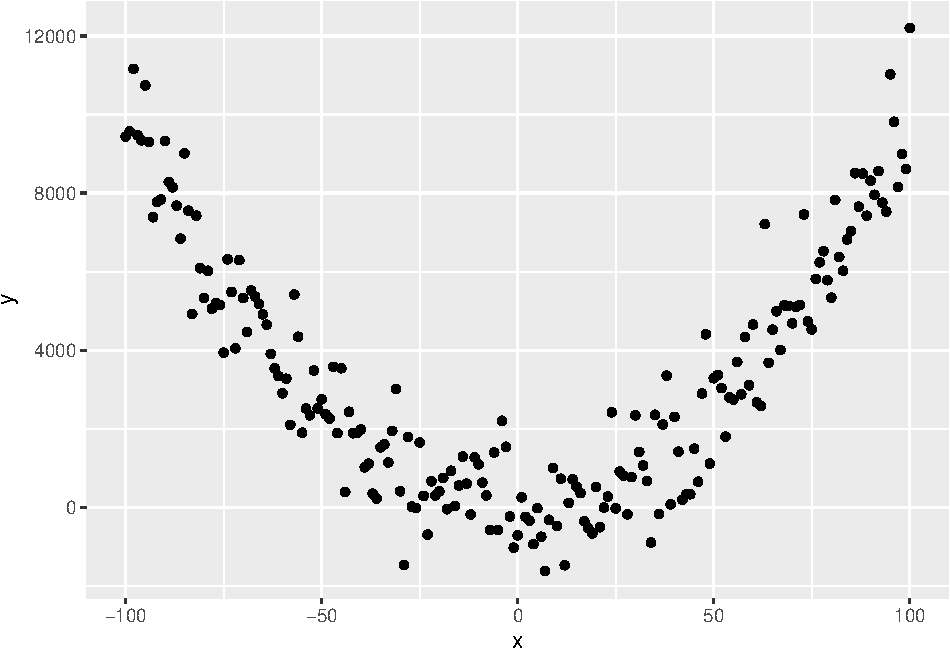
\includegraphics{Experimental-Design,-ANOVA-and-ANCOVA_files/figure-latex/unnamed-chunk-2-1.pdf}

How, you ask!? Well\ldots. consider this equation:

\(y = 0.01 + x + x^{2} + \epsilon\)

Referring to our generic model structure above,

\(y = \beta_{0}+\beta_{1}*X_{1}+\beta_{2}*X_{2}+\epsilon\)

we hopefully can see that \(\beta_{0} = 0.01\), \(\beta_{1} = 0\) and \(\beta_{2} = 1\), where \(X_{2} = X^{2}\)!

Linear models are perfectly capable of being used to estimate non-linear relationships!

Here is the code to make that figure.

\begin{Shaded}
\begin{Highlighting}[]
\CommentTok{\# set x range}
\NormalTok{x }\OtherTok{\textless{}{-}} \SpecialCharTok{{-}}\DecValTok{100}\SpecialCharTok{:}\DecValTok{100}
\CommentTok{\# define y without error}
\NormalTok{y\_det }\OtherTok{\textless{}{-}} \FloatTok{0.01}\SpecialCharTok{+}\NormalTok{x}\SpecialCharTok{\^{}}\DecValTok{2}
\CommentTok{\# add some random variation}
\NormalTok{y }\OtherTok{\textless{}{-}}\NormalTok{ y\_det}\SpecialCharTok{+}\FunctionTok{rnorm}\NormalTok{(}\FunctionTok{length}\NormalTok{(x),}\DecValTok{0}\NormalTok{,}\DecValTok{1000}\NormalTok{)}

\CommentTok{\# create dataframe and plot}
\NormalTok{df }\OtherTok{\textless{}{-}} \FunctionTok{data.frame}\NormalTok{(x, y)}
\FunctionTok{ggplot}\NormalTok{(df, }\FunctionTok{aes}\NormalTok{(}\AttributeTok{x =}\NormalTok{ x, }\AttributeTok{y =}\NormalTok{ y))}\SpecialCharTok{+}
  \FunctionTok{geom\_point}\NormalTok{()}
\end{Highlighting}
\end{Shaded}

\hypertarget{readings--}{%
\chapter{Readings ----}\label{readings--}}

There are several resources that will help with this section of the stats course, and onwards

\begin{itemize}
\tightlist
\item
  Getting Started with R - An Introducton for Biologists, Second Edition (available as an electronic online resource via StarPlus). Specifically Chapter 5 and 6.
\item
  Experimental Design for the Life Sciences - Nick Colegrave and Graham Ruxton (seen on eBay for £2.50!)
\item
  Of course, the venerable coursebook for APS 240: \url{https://dzchilds.github.io/stats-for-bio/index.html}
\end{itemize}

\hypertarget{install-some-extra-packages--}{%
\section{Install some extra packages ----}\label{install-some-extra-packages--}}

In order to make this module more effective, we are going to use some additional resources from CRAN.

Please install these packages, if you have not already, using the install packages tab in RStudio:

\begin{itemize}
\tightlist
\item
  \texttt{tidyverse}
\item
  \texttt{ggfortify}
\item
  \texttt{agricolae}
\item
  \texttt{car}
\item
  \texttt{gmodels}
\item
  \texttt{visreg}
\item
  \texttt{patchwork}
\end{itemize}

\hypertarget{introduction-to-experimental-design}{%
\chapter{Introduction To Experimental Design}\label{introduction-to-experimental-design}}

Experiments help us answer questions, but there are also non-experimental techniques. What is so special about experiments?

One of the central features of an experiment is the \emph{treatment} - a manipulation of some variable of interest that should have an effect on the response variable we are investigating. Whether you are manipulating the levels of a hormone to explore it's impact on a cell/organ or embryo development, the concentration of a drug to explore it's efficancy in treating a disease or the levels of nitrogen in soil to explore the impacts on plant growth, a treatment is a deliberate manipulation.

It is also important to remember that there can be \emph{natural} treatments - there may be natural variation among cells, organisms or gradients in the environment that you can use to represent treatments.

So, to be very clear:

\begin{enumerate}
\def\labelenumi{\arabic{enumi}.}
\tightlist
\item
  Experiments allow us to set up a direct comparison among the \emph{levels} or \emph{values} of \emph{treatments} of interest.
\item
  We can design experiments to minimize any bias in the comparison.
\item
  We can design experiments so that the error in the comparison is small.
\item
  We design experiments to be in control, and having that control allows us to make stronger inferences about the nature of differences that we see in the response variable.
\end{enumerate}

\begin{quote}
Experiments allow us to move towards making inferences about causation.
\end{quote}

This last point distinguishes an experiment from an observational study. In an observational study we merely observe which units are in which treatment groups; we don't get to \emph{control that assignment}. This underpins the classic issue with assigning \emph{causation to correlation} - in the following two examples, there is a strong association between the variables, but there has been no control/manipulation.

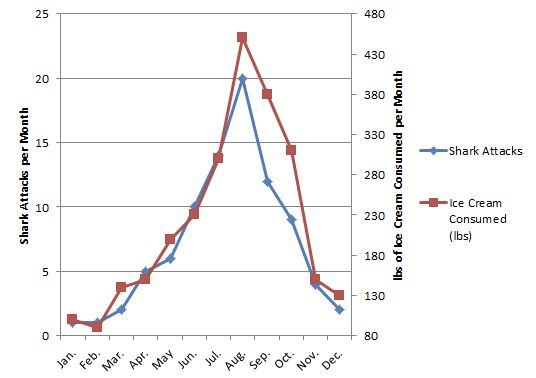
\includegraphics[width=7.44in]{images/IceCream_Shark}
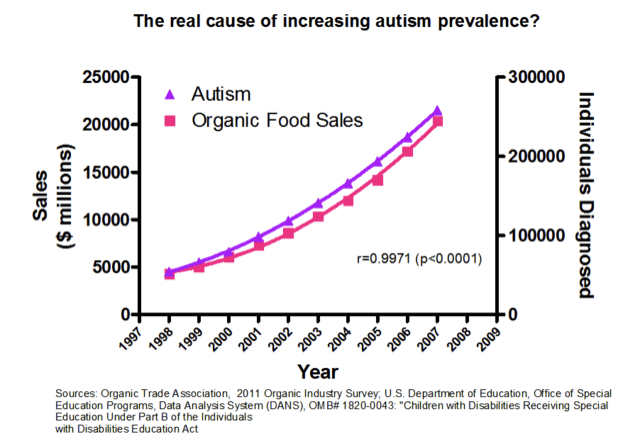
\includegraphics[width=8.89in]{images/Autism_Organic}

\hypertarget{conepts-associated-with-causation}{%
\section{Conepts associated with causation}\label{conepts-associated-with-causation}}

Mosteller and Tukey (1977) list three concepts associated with causation and state that at least two (preferably all three) are needed to support a causal relationship:

\begin{itemize}
\tightlist
\item
  \emph{Consistency} -- make a change and the response is in the same direction or the amount of response is \emph{consistent} across populations
\item
  \emph{Responsiveness} -- make a change and the response changes according to theory
\item
  \emph{Mechanism} -- make a change and we can monitor/identify a mechanism leading from cause to effect
\end{itemize}

Let's look at a classic example. Smoking and lung cancer -- from 1922 to 1947 annual deaths for lung cancer went from 612 to 9287 (Observation). This was thought in the 1950s to be either an effect of smoking tobacco or atmospheric pollution (Hypothesis). Numerous studies showed that lung cancer was more prevalent in smokers (Observation: \emph{consistency}). Chemical analyses of tobacco showed it contained carcinogens (Association: \emph{mechanism}). Public health programs resulted in a reduction in smoking and lung cancer rates decreased (Intervention: \emph{responsiveness}).

Note the initial study was an observational study and in this case it was not ethical to do the experiment per se!

\hypertarget{components-of-an-experiment}{%
\section{Components of an Experiment}\label{components-of-an-experiment}}

An experiment has \emph{treatments, experimental units, responses, and a method to assign treatments to units}. These four things specify the experimental design.

Not all experimental designs are created equal. A good experimental design must adhere to the 3Rs. It should reveal consistency, responsiveness and mechanism. The way this happens is by avoiding systematic error in measuring things, and allow estimation of error in measurements with precision.

\hypertarget{the-holy-grail-of-a-control}{%
\section{The holy grail of a control}\label{the-holy-grail-of-a-control}}

At this point, it would be good to revisit the APS 240 sections \href{https://dzchilds.github.io/stats-for-bio/principles-experimental-design.html\#experimental-control}{on controls} and \href{https://dzchilds.github.io/stats-for-bio/principles-experimental-design.html\#EXPT-DESIGN-PROCEDURAL-CONTROLS}{procedural controls}

\hypertarget{so-what-does-a-good-experimental-design-do}{%
\section{So what does a good experimental design do?}\label{so-what-does-a-good-experimental-design-do}}

In short, a good experimental design must:

\begin{itemize}
\tightlist
\item
  Avoid systematic error
\item
  Allow estimation of error
\item
  Be precise
\item
  Have broad validity.
\end{itemize}

Lets walk through some definitions.

If our experiment has \emph{systematic error}, then our comparisons will be biased, no matter how precise our measurements are or how many experimental units we use. \textbf{Randomisation} is our tool to combat \emph{systematic error}.

Even without \emph{systematic error}, there will be random error in the responses - this is what we call variation in what we are measuring or more formally variance. Such variation in responses invariably leads to random error in the treatment comparisons. When we compared two means in the t-test, we had to deal with the variation in both groups!

Experiments are precise when this random error in the treatment comparisons is small. Precision depends on the size of the random errors in the responses, the number of units used (\textbf{replication}), and the experimental design used.

Experiments must be designed so that we have an estimate of the size of random error. This permits statistical inference: for example, confidence intervals (which arise from standard errors) or tests of significance based on t- or F-statistics.

We cannot do inference without an estimate of this variation. We would like our conclusions to be valid for a wide population, so we need to \emph{randomise} our subjects or objects we are measuring - for example, we may need to be aware of both sexes and of young and old individuals. But there are always compromises - for example, broadening the scope of validity by using a variety of experimental units may decrease the precision of the responses.

\hypertarget{how-do-we-increase-precision-and-reduce-bias}{%
\section{How do we increase precision and reduce bias?}\label{how-do-we-increase-precision-and-reduce-bias}}

There are several key concepts

\hypertarget{blinding}{%
\subsection{Blinding}\label{blinding}}

\emph{Blinding} occurs when the evaluators of a response do not know which treatment was given to which unit. Blinding helps prevent bias in the evaluation, even unconscious bias from well-intentioned evaluators. Double blinding occurs when both the evaluators of the response and the (human subject) experimental units do not know the assignment of treatments to units. Blinding the subjects can also prevent bias, because subject responses can change when subjects have expectations for certain treatments.

\hypertarget{placebos}{%
\subsection{Placebos}\label{placebos}}

\emph{Placebo} is a null treatment that is used when the \emph{act} of applying a treatment--- any treatment --- has an effect. Placebos are often used with human subjects, because people often respond to the process of receiving any treatment: for example,
reduction in headache pain when given a sugar pill. Blinding is important when placebos are used with human subjects. Placebos are also useful for nonhuman subjects. The apparatus for spraying a field with a pesticide may compact the soil. Thus we drive the apparatus over the field, without actually spraying, as a placebo treatment.

\hypertarget{confounders}{%
\subsection{Confounders}\label{confounders}}

\emph{Confounding} occurs when the effect of one factor or treatment cannot be distinguished from that of another factor or treatment. The two factors or treatments are said to be confounded. Except in very special circumstances, confounding should be avoided. Consider the following example. We plant corn variety A in Yorkshire and corn variety B in Lancashire. In this experiment, we cannot distinguish location effects (Yorkshire vs.~Lancashire) from variety effects (cornA vs.~cornB) --- the variety factor and the location factor are confounded.

This is despite the fact that we know that Yorkshire will be better\ldots. (that's a joke)

\hypertarget{experimental-vs.-measurement-units}{%
\section{Experimental vs.~Measurement units}\label{experimental-vs.-measurement-units}}

A common source of difficulty in designing experiments is the distinction between experimental units and measurement units. We need to know the experimental units, as this is the key value used to generate our inference.

Now is a good time to re-look at the short section on \href{https://dzchilds.github.io/stats-for-bio/principles-experimental-design.html\#jargon-busting}{Jargon Busting} from the APS 240 book.

\hypertarget{experimental-and-measurement-units-an-example}{%
\subsection{Experimental and measurement units: an example}\label{experimental-and-measurement-units-an-example}}

Consider an educational study, with six classrooms of 25 pupils. Each classroom of students is then assigned, at random, to one of two different reading programmes.

At the end of a six-week term, all the students are evaluated via a common reading exam.

\hypertarget{the-challenge-question}{%
\subsubsection{The challenge question}\label{the-challenge-question}}

\begin{quote}
Are there six experimental units (the classrooms) or 150 (25*6; the students)? We measured the reading ability of the students\ldots{} but they were in classroom sets of 25\ldots.
\end{quote}

\hypertarget{identifying-the-experimental-unit---an-example-of-pseudo-replication}{%
\subsection{\texorpdfstring{Identifying the experimental unit - an example of \textbf{pseudo-replication}}{Identifying the experimental unit - an example of pseudo-replication}}\label{identifying-the-experimental-unit---an-example-of-pseudo-replication}}

To identify the experimental units the key question is: To which \emph{thing} (students or classrooms) did we randomly allocate our treatments?

If we randomly allocated reading programmes to students, then students would be the experimental units. But we didn't, so the classroom is the experimental unit -- it is the classroom to which we randomly allocated treatments.

\emph{The classroom is the experimental unit}.

However, you are right - we don't \emph{measure} how a classroom reads; we measure how students read. Thus \emph{students are the measurement units} for this experiment.

\hypertarget{psudo-replication}{%
\subsection{Psudo-replication}\label{psudo-replication}}

Confusing these two things can lead to \textbf{pseudo-replication}. Treating measurement units as experimental usually leads to overoptimistic analysis --- we will reject null hypotheses more often than we should, and our confidence intervals will be too narrow. The usual way around this is to determine a single response for each experimental unit.

There is additional information on \href{https://dzchilds.github.io/stats-for-bio/principles-experimental-design.html\#independence}{Independence and Pseudoreplication} in the the APS 240 book.

\hypertarget{independence-and-example}{%
\subsubsection{Independence: and example}\label{independence-and-example}}

Consider an experiment with two growth chambers each containing 100 plants. One of the chambers received enhanced C02. One night after collecting data you leave the door open on the C02 chamber and the temperature drops and so the plants grow more slowly. When you come to analyze the data you get a highly significant effect of slow growth. However, that C02 results in reduced plant growth not what you expect (CO2 is good for photosynthesis\ldots).

This is an entirely plausible outcome caused by misallocating plants as the experimental unit - it was really the CO2 chamber\ldots{} to avoid such problems, one needs many chambers.

Consider a second experiment where you have 200 growth chambers and randomly allocate plants to each. If you \emph{forget to close one door} it really has no effect as just one plant is affected. In fact, to get the same effect as in the first experiment you would have to accidentally leave the doors open on all 100 of the elevated C02 chambers. This is very unlikely indeed!!!

\begin{quote}
There are 9 x 1058 ways selecting 100 chambers from 200 chambers so the chance of accidentally picking all the elevated C02 chambers is 1/ 9x10580 (stars in universe 7 x 1022).
\end{quote}

Proper \textbf{randomization} and \textbf{replication} is very different from \textbf{pseudo-replication}.

\hypertarget{randomization-with-replication-protects-against-confounding}{%
\subsection{Randomization with Replication protects against Confounding}\label{randomization-with-replication-protects-against-confounding}}

An experiment is properly randomized if the method for assigning treatments to units involves a known, well-understood probabilistic scheme. The probabilistic scheme is called a randomization.

\begin{quote}
In general, more experimental units with fewer measurement units per experimental unit works better.
\end{quote}

No matter which features of the population of experimental units are associated with our response, our randomizations should put approximately \emph{half the individuals with these features} into \emph{each treatment group}.

Recall our example above of considering sex and age of subjects and imagine a treatment with two levels (hot and cold). Done well, proper randomisation will put approximately half the males, half the females, half the older, half the younger etc into each of the treatment levels.

The beauty of randomization is that it helps prevent \emph{confounding}, even for factors that we do not know are important.

\hypertarget{haphazard-is-not-randomized---beware-the-non-randomized-experiment}{%
\subsection{\texorpdfstring{\textbf{haphazard} is NOT randomized - beware the non-randomized experiment --}{haphazard is NOT randomized - beware the non-randomized experiment --}}\label{haphazard-is-not-randomized---beware-the-non-randomized-experiment}}

A company is evaluating two different word processing packages for use by its clerical staff. Part of the evaluation is how quickly a test document can be entered correctly using the two programs. We have 20 test secretaries, and each secretary will enter the document twice, using each programme once.

Suppose that all secretaries did the evaluation in the order A first and B second. Does the second programme have an advantage because the secretary will be familiar with the document and thus enter it faster? Or maybe the second programme will be at a disadvantage because the secretary will be tired and thus slower?

Randomization generally costs little in time and trouble, but it can save us from \texttt{disaster}. The experiment above needs secretaries randomly assigned to A first -\textgreater{} B second and B first -\textgreater{} A second (50\% in each!).

Anything that might affect your responses should be \emph{randomized}! For example

\begin{itemize}
\tightlist
\item
  If the experimental units are not used simultaneously, you can (should) randomize the order in which they are used.
\item
  If the experimental units are not used at the same location, you can (should) randomize the locations at which they are used.
\item
  If you use more than one measuring instrument for determining response, you can (should) randomize which units are measured on which instruments.
\end{itemize}

\hypertarget{mini-quiz}{%
\section{Mini-Quiz}\label{mini-quiz}}

\begin{quote}
A PhD student want to determine the effects of protein on beetle reproduction, so they design an experiment with a control and protein enhanced diet. To assign beetles to each of the treatments they pour a culture onto the table and catch the first 30 beetles that run to the edge of the table, these receive the protein enhanced diet. The next 30 beetles go in the control. \textbf{Is this randomized?}
\end{quote}

(Hmm \ldots. is there anything about the first 30 beetles that reach the edge of the table that could \emph{bias} your inference?)

\hypertarget{replication-how-many}{%
\section{Replication: How many?}\label{replication-how-many}}

There is a really common question that people ask. How many replicates do I need? Unfortunatly, there are no simple rules\ldots{} it depends\ldots{} on\ldots.

\begin{itemize}
\tightlist
\item
  Resources available (\$/£/€ and equipment and time)
\item
  Variability of experimental units
\item
  Treatment structure
\item
  Size of effect (response)
\item
  Relative importance of different comparisons
\end{itemize}

There is, however, a set of tools that can help with estimating sample sizes. It's called power analysis and requires that you have some a priori estimate of the expected variation in your response variable.

\hypertarget{examples-and-challenge-questions}{%
\chapter{Examples and Challenge Questions}\label{examples-and-challenge-questions}}

In this section, we will review a field based experimental design example. There are challenge questions to answer.

We will also introduce tools to generate randomised experimental designs - this is a good trick to have up your sleeves!

\hypertarget{designing-your-first-experiment}{%
\section{Designing your first experiment}\label{designing-your-first-experiment}}

You are challenged to design an Arctic field manipulation experiment to evaluate UV-B radiation and increased CO2 impacts on plant growth.

Context: an arctic tundra study
Increasing ultraviolet-B (+UV-B) radiation from ozone depletion (the arctic ozone hole)
Increasing atmospheric CO2 (+CO2) from anthropogenic emissions
For plants: +UV-B potentially harmful, +CO2 potentially beneficial

Hypotheses
Elevated (+) UV-B radiation will reduce the growth of arctic plants
Elevated (+) \(CO_{2}\) will increase the growth of arctic plants

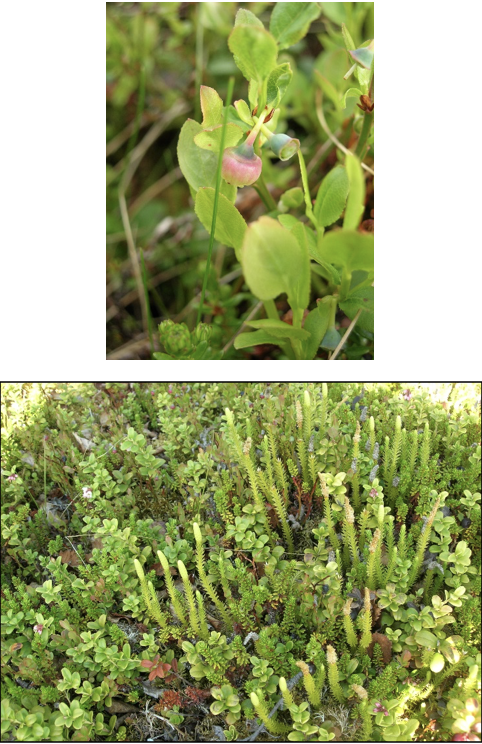
\includegraphics[width=6.69in]{images/ArcticPlants}

The resources available to you are constrained. The arctic research station has given permission for 16 plots (each 2m x 2m) in the natural vegetation nearby.

One +UV-B plot (2m x 2m) costs £4000 (this provides the UV-B lamps, frame, power and control system, wooden walkways around the plots)
One \(+CO_{2}\) plot (2m x 2m) costs £6000 (this provides a CO2 release system, CO2 control and covers CO2 purchase costs, wooden walkways around the plots)
One control plot (2m x 2m) costs £200 (marking posts, wooden walkways around the plots)

You have a budget of £61,000

Design an experiment to test the hypotheses (i.e.~the design of the plots and treatments including replication, not what measurements you will take - which will be plant growth rates\ldots.). Think hard about this. How many treatments do you have? How many plots/treatment would you like to allocate? Is this possible? Will this be a balanced design, given your max budget? If it isn't, what rule can you use to allocate them replicates to treatments?

Write an answer down, before moving to the next section. We'll provide the answer separately!

\hypertarget{design-and-analysis-of-experiments}{%
\chapter{Design and Analysis of Experiments}\label{design-and-analysis-of-experiments}}

In this section we are going to learn about how to implement two experimental designs:

\begin{itemize}
\tightlist
\item
  CRD: the completely randomised design
\item
  CRBD: the completely randomised block design.
\end{itemize}

These two designs are valuable in dealing with two things that make it hard to make strong inference from experiments: \emph{noise} and \emph{counfounding effects}.

These unwated sources of variation comes in two forms (see \href{https://dzchilds.github.io/stats-for-bio/principles-experimental-design.html\#confounded-and-noisy-experiments}{APS 240 reading})

\begin{enumerate}
\def\labelenumi{\arabic{enumi}.}
\item
  The first is \emph{confounding variation}. This occurs when there are one or more other sources of variation that work in parallel to the factor we are investigating and make it hard, or impossible, to unambiguously attribute any effects we see to a single cause. Confounding variation is particularly problematic in observational studies because, by definition, we don't manipulate the factors we're interested in.
\item
  The second is \emph{noise}. This describes variation that is unrelated to the factor we are investigating but adds variability to the results so that it is harder to see, and detect statistically, any effect of that factor. As noted above, much of experimental design is about improving our ability to account for noise in a statistical analysis.
\end{enumerate}

We will consider these together, as some of the techniques for dealing with them are be applicable to both. The primary tools for dealing with them are

\begin{enumerate}
\def\labelenumi{\arabic{enumi}.}
\tightlist
\item
  randomisation
\item
  blocking
\item
  appropriate controls
\item
  additional treatments.
\end{enumerate}

In the following sections, we are going to focus on the first three. In doing so, we will also revisit how we make inference from 1-way ANOVA experiments and introduce a more generalised approach to making \emph{contrasts} we want. If you recall from the 1-way ANOVA work you did in the previous module (Week 7), we learned about \emph{treatment contrasts}, the default comparison of means to a reference level, and then the \emph{Tukey test}, which makes all pairwise comparisons. Here will will find an intermediate zone.

\hypertarget{a-crd-completely-randomised-design-example}{%
\section{A CRD (Completely Randomised Design) Example}\label{a-crd-completely-randomised-design-example}}

The experiment is about plant crop biomass yield under several herbicide treatments - the herbicide targets weeds and not our target plant (e.g.~Glyphosate): a control and two herbicides, and a third treatment that is a placebo - applied water but no herbicide.

The data for this example are called \texttt{plantYield.csv}.

For each treatment, we have n = 30 plants in separate pots in standarised conditions.

Can you explain why we are using the placebo? Do you know the measurement and experimental unit? As this is a 1-way ANOVA, what is the baseline hypothesis? Given that there is a control and two herbicides, are there alternative hypotheses you might test?

Let's look at the structure of the design. As hoped, we have 30 replicates of each treatment. The second view reveals that the replicates are allocated randomly among the replicate plants. There is no order to the values in the \texttt{treat} column.

\begin{verbatim}
## treat
##    Cont   Herb1   Herb2 Placebo 
##      30      30      30      30
\end{verbatim}

\begin{verbatim}
##    plots r   treat
## 1      1 1 Placebo
## 2      2 2 Placebo
## 3      3 1    Cont
## 4      4 3 Placebo
## 5      5 1   Herb2
## 6      6 2    Cont
## 7      7 1   Herb1
## 8      8 2   Herb2
## 9      9 3    Cont
## 10    10 4 Placebo
\end{verbatim}

We have now added data to this design in order to start doing statistics. The \emph{TRUTH} of these data are that on average, the controls have a yield of 20, Herbicide 1 increases yield by 5, Herbicide 2 by 6 and the placebo by 1 unit. These data are also quite variable. The standard deviation around the yields is large. We are going to analyse these data and

\begin{enumerate}
\def\labelenumi{\arabic{enumi}.}
\tightlist
\item
  see if we can recover these estimates of `known' yield.
\item
  test the null hypothesis.
\item
  test the hypothesis that herbicides, on average, increase yield.
\item
  test whether the two herbicides are different.
\item
  test whether the placebo is different from the control.
\end{enumerate}

And there is the answer to one of the questions above!

\begin{Shaded}
\begin{Highlighting}[]
\CommentTok{\# look at the design now.}
\FunctionTok{head}\NormalTok{(plantYield)}
\end{Highlighting}
\end{Shaded}

\begin{verbatim}
##   plots r   treat      obs
## 1     1 1 Placebo 27.54449
## 2     2 2 Placebo 22.39018
## 3     3 1    Cont 18.23051
## 4     4 3 Placebo 19.79473
## 5     5 1   Herb2 23.46557
## 6     6 2    Cont 21.65736
\end{verbatim}

\hypertarget{the-dplyr-and-ggplot-pipeline-for-inference.}{%
\subsection{The dplyr and ggplot pipeline for inference.}\label{the-dplyr-and-ggplot-pipeline-for-inference.}}

Now we can move to our standard data management and visualisation pipeline.

\begin{enumerate}
\def\labelenumi{\arabic{enumi}.}
\tightlist
\item
  review the data (the \texttt{plantYield.csv} file contains the data)
\item
  sumamrise the data with dplyr - generate means and se's for the treatments
\item
  visualise with ggplot2
\end{enumerate}

\begin{Shaded}
\begin{Highlighting}[]
\CommentTok{\# check the data}
\CommentTok{\# note}
\CommentTok{\# obs == yield}
\CommentTok{\# treat == treatment}
\CommentTok{\# r = replicate (there are 30 of each treatment)}

\FunctionTok{glimpse}\NormalTok{(plantYield)}
\end{Highlighting}
\end{Shaded}

\begin{verbatim}
## Rows: 120
## Columns: 4
## $ plots <dbl> 1, 2, 3, 4, 5, 6, 7, 8, 9, 10, 11, 12, 13, 14, 15, 16, 17, 18, 1~
## $ r     <int> 1, 2, 1, 3, 1, 2, 1, 2, 3, 4, 5, 4, 6, 5, 3, 2, 6, 7, 8, 4, 5, 3~
## $ treat <chr> "Placebo", "Placebo", "Cont", "Placebo", "Herb2", "Cont", "Herb1~
## $ obs   <dbl> 27.54449, 22.39018, 18.23051, 19.79473, 23.46557, 21.65736, 26.5~
\end{verbatim}

\begin{Shaded}
\begin{Highlighting}[]
\CommentTok{\# let\textquotesingle{}s force treat to be a factor.  This will make life easier later...}
\NormalTok{plantYield }\OtherTok{\textless{}{-}}\NormalTok{ plantYield }\SpecialCharTok{\%\textgreater{}\%} 
  \FunctionTok{mutate}\NormalTok{(}\AttributeTok{treat =} \FunctionTok{factor}\NormalTok{(treat))}

\CommentTok{\# summarise to get means and ses}
\NormalTok{sumDat }\OtherTok{\textless{}{-}}\NormalTok{ plantYield }\SpecialCharTok{\%\textgreater{}\%} 
  \FunctionTok{group\_by}\NormalTok{(treat) }\SpecialCharTok{\%\textgreater{}\%} 
  \FunctionTok{summarise}\NormalTok{(}
    \CommentTok{\# calculate the means}
    \AttributeTok{meanYield =} \FunctionTok{mean}\NormalTok{(obs),}
    \CommentTok{\# calculate the se}
    \AttributeTok{seYield =} \FunctionTok{sd}\NormalTok{(obs)}\SpecialCharTok{/}\FunctionTok{sqrt}\NormalTok{(}\FunctionTok{n}\NormalTok{())}
\NormalTok{  )}

\CommentTok{\# plot the raw data and the mean±se}
\CommentTok{\# start with the mean±se and then add the raw data}
\FunctionTok{ggplot}\NormalTok{(sumDat, }\FunctionTok{aes}\NormalTok{(}\AttributeTok{x =}\NormalTok{ treat, }\AttributeTok{y =}\NormalTok{ meanYield))}\SpecialCharTok{+}
  \FunctionTok{geom\_point}\NormalTok{(}\AttributeTok{size =} \DecValTok{5}\NormalTok{)}\SpecialCharTok{+}
  \FunctionTok{geom\_errorbar}\NormalTok{(}\AttributeTok{data =}\NormalTok{ sumDat, }\FunctionTok{aes}\NormalTok{(}\AttributeTok{ymin =}\NormalTok{ meanYield }\SpecialCharTok{{-}}\NormalTok{ seYield, }\AttributeTok{ymax =}\NormalTok{ meanYield}\SpecialCharTok{+}\NormalTok{seYield),}
                \AttributeTok{width =} \FloatTok{0.1}\NormalTok{)}\SpecialCharTok{+}
  \FunctionTok{geom\_point}\NormalTok{(}\AttributeTok{data =}\NormalTok{ design, }\FunctionTok{aes}\NormalTok{(}\AttributeTok{x =}\NormalTok{ treat, }\AttributeTok{y =}\NormalTok{ obs), }\AttributeTok{colour =} \StringTok{\textquotesingle{}red\textquotesingle{}}\NormalTok{, }\AttributeTok{alpha =} \FloatTok{0.3}\NormalTok{)}
\end{Highlighting}
\end{Shaded}

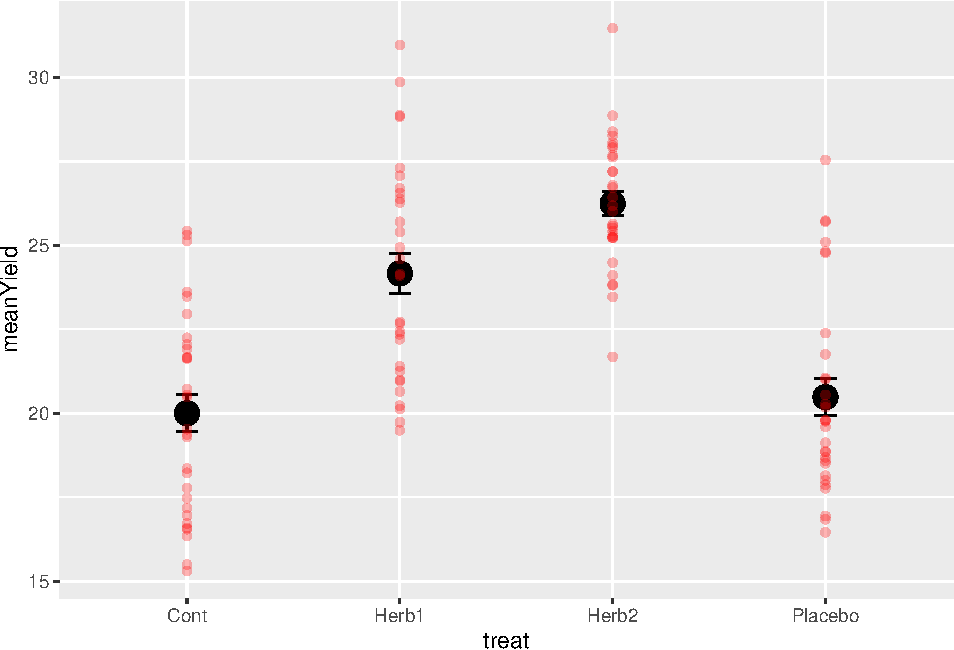
\includegraphics{Experimental-Design,-ANOVA-and-ANCOVA_files/figure-latex/unnamed-chunk-10-1.pdf}

A few things to notice.

\begin{enumerate}
\def\labelenumi{\arabic{enumi}.}
\tightlist
\item
  The data are quite variable and the means of the herbicide treatments are roughly 5 and 6 units higher than the control. GOOD. This is as we expected\ldots.
\item
  The standard errors are quite small, even though the variation is large! Why is that!?
\item
  The two herbicides don't look very different, especially given the variation around each treatment. Neither do the placebo and control. We need some stats.
\item
  For those of you interested in some extra reading and thinking, the 95\% Confidence Interval around the means can be calculated using \(1.96*SE` == `1.96*sd(obs)/sqrt(n())\). Go ahead and do that and look into that if you want\ldots{}
\end{enumerate}

\hypertarget{the-one-way-anova.}{%
\subsection{The One-Way ANOVA.}\label{the-one-way-anova.}}

If you've been paying attention, we've essentially designed and plotted the data for a 1-way ANOVA. These data are very similar to the daphnia parasite data we finished semester 1 with.

To analyse these data, we use the \texttt{lm()} function to build the model, check assumptions, and then make inference. Let's go.

\begin{Shaded}
\begin{Highlighting}[]
\CommentTok{\# the model}
\NormalTok{modYield }\OtherTok{\textless{}{-}} \FunctionTok{lm}\NormalTok{(obs }\SpecialCharTok{\textasciitilde{}}\NormalTok{ treat, }\AttributeTok{data =}\NormalTok{ plantYield)}

\CommentTok{\# assumptions}
\FunctionTok{autoplot}\NormalTok{(modYield)}
\end{Highlighting}
\end{Shaded}

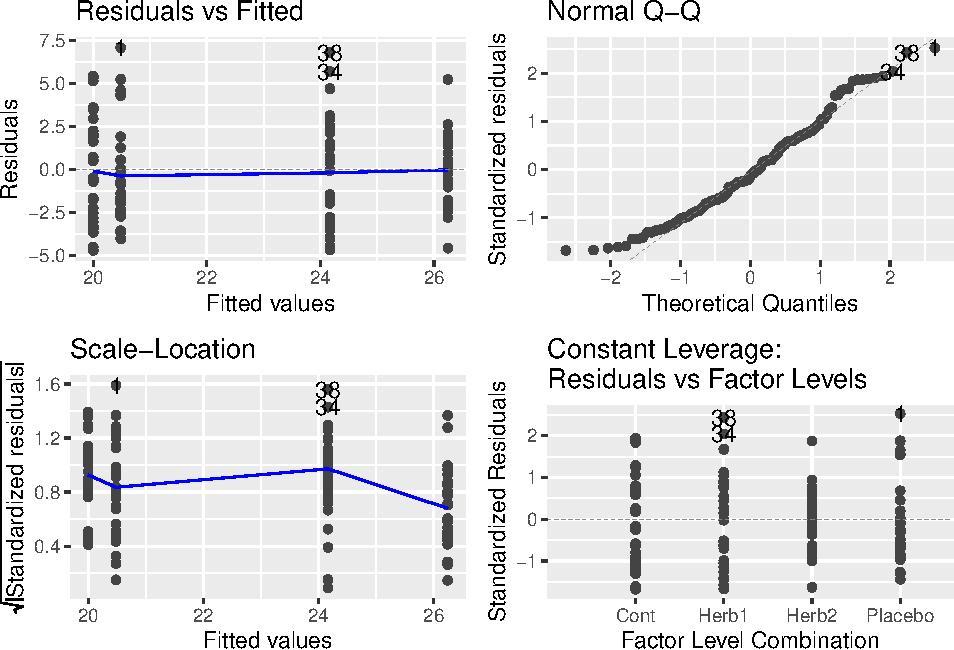
\includegraphics{Experimental-Design,-ANOVA-and-ANCOVA_files/figure-latex/unnamed-chunk-11-1.pdf}

\begin{Shaded}
\begin{Highlighting}[]
\CommentTok{\# inference: anova}
\FunctionTok{anova}\NormalTok{(modYield)}
\end{Highlighting}
\end{Shaded}

\begin{verbatim}
## Analysis of Variance Table
## 
## Response: obs
##            Df Sum Sq Mean Sq F value    Pr(>F)    
## treat       3 807.49 269.164  33.257 1.383e-15 ***
## Residuals 116 938.85   8.094                      
## ---
## Signif. codes:  0 '***' 0.001 '**' 0.01 '*' 0.05 '.' 0.1 ' ' 1
\end{verbatim}

\begin{Shaded}
\begin{Highlighting}[]
\CommentTok{\# contrasts}
\FunctionTok{summary}\NormalTok{(modYield)}
\end{Highlighting}
\end{Shaded}

\begin{verbatim}
## 
## Call:
## lm(formula = obs ~ treat, data = plantYield)
## 
## Residuals:
##     Min      1Q  Median      3Q     Max 
## -4.6952 -2.1542 -0.3872  1.8383  7.0609 
## 
## Coefficients:
##              Estimate Std. Error t value Pr(>|t|)    
## (Intercept)   20.0004     0.5194  38.506  < 2e-16 ***
## treatHerb1     4.1655     0.7346   5.671 1.06e-07 ***
## treatHerb2     6.2449     0.7346   8.502 7.43e-14 ***
## treatPlacebo   0.4832     0.7346   0.658    0.512    
## ---
## Signif. codes:  0 '***' 0.001 '**' 0.01 '*' 0.05 '.' 0.1 ' ' 1
## 
## Residual standard error: 2.845 on 116 degrees of freedom
## Multiple R-squared:  0.4624, Adjusted R-squared:  0.4485 
## F-statistic: 33.26 on 3 and 116 DF,  p-value: 1.383e-15
\end{verbatim}

\hypertarget{making-insight-and-inference}{%
\subsection{Making insight and inference}\label{making-insight-and-inference}}

Lets walks through things very discretely.

\begin{enumerate}
\def\labelenumi{\arabic{enumi}.}
\tightlist
\item
  Our graph suggests that herbicide treatments have an effect of increasing yield.
\item
  Our model is designed to test this hypothesis - are any of the differences among means non-zero?
\item
  Our hypothesis is probably really about whether the herbicide and placebos are different than the controls. All Hail the \emph{treatment contrast}!
\item
  Our diagnostics are fantastic\ldots{} the best you've ever seen.
\item
  The Anova Table confirms that there are differences - we can reject the null hypothesis
\item
  The summary table confirms that Herb1 and Herb2 are both larger than controls and the Placebo is not.
\end{enumerate}

How do we interpret even more?

The estimate associated with Control is 20! Just where it should be.

The estimates associated with Herb1, Herb2 and Placebo are the differences between the mean of these treatments and the control (the reference level!). These differences are positive for Herb1 and Herb2, close to 5 and 6 respectively (as expected) and this positive difference is not 0 via the statistical test.

However, the difference for Placebo is close to 0 and therefore we can not reject the null hypothesis test that it differs from control. GENUIS!

\hypertarget{a-priori-vs.-post-hoc-contrasts}{%
\section{A priori vs.~Post-Hoc Contrasts}\label{a-priori-vs.-post-hoc-contrasts}}

As we discussed above, there are likely several other questions we might have wanted to answer when designing this experiment. For example, are the two herbicides different in their effects?

\hypertarget{custom-contrasts-versus-the-tukey-test}{%
\subsection{Custom contrasts versus the Tukey Test}\label{custom-contrasts-versus-the-tukey-test}}

In the semester 1, we introduced how to do a Tukey Test. This is known as an \emph{a posteriori} test -- testing the significance of things suggested by the experiment, also known as data snooping or data dredging. These are multiple comparison methods (Bonferroni, Scheffe method, Tukey honest significant difference, Duncan's multiple range test) which try to control the chance of getting a significant result by chance.

To understand the risks of these, consider this experimental design. We have 7 treatments. With 7 treatments, there are 21 pairwise comparisons. With p-value threshold of \(0.05\) we expect 1/20 (5/100) tests to be significant. So with this 7 treatment and 21 comparison design, would you expect a signficant result by chance? You betyja.

This is why, unless a priori (in advance) you can justify ALL pairwise comparisons, a Tukey Test may not be appropriate.

Some statisticians really don't like them:

\begin{quote}
``In my view multiple comparison methods have no place at all in the interpretation of data'' -Nelder (a very very very well respected statistician).
\end{quote}

\hypertarget{the-more-appropriate-approach---custom-contrasts}{%
\subsubsection{The more appropriate approach - custom contrasts}\label{the-more-appropriate-approach---custom-contrasts}}

The \emph{more appropriate} approach is to specify \emph{a priori} (before the experiment) a set of hypotheses you want to test, and then test them using contrasts.

For our experiment, as noted above, we were probably interested in what our treatment contrasts provided - tests of difference with the control. But we had a few others too.

Specifying specific contrasts is easy once you get your head around the `structure' of the syntax.

Lets have a go with specifying a comparison JUST between Herbicide 1 and the control. Remember that your model is called \texttt{modYield} and your data is called \texttt{design}.

\begin{Shaded}
\begin{Highlighting}[]
\CommentTok{\# check the levels and ORDERING of the treatments}
\CommentTok{\# this function, levels(), tells you this}
\CommentTok{\# note the ORDER: it is alphabetical, and control comes first}
\CommentTok{\# the words fill in four slots c(X,X,X,X). }
\CommentTok{\# we will use these slots....}
\FunctionTok{levels}\NormalTok{(plantYield}\SpecialCharTok{$}\NormalTok{treat)}
\end{Highlighting}
\end{Shaded}

\begin{verbatim}
## [1] "Cont"    "Herb1"   "Herb2"   "Placebo"
\end{verbatim}

\begin{Shaded}
\begin{Highlighting}[]
\CommentTok{\# define the contrast you want using {-}1, 1 and 0\textquotesingle{}s}
\CommentTok{\# this says compare control with herbicide 1.... and ignore the Herb2 and Placebo}
\CommentTok{\# we give the reference {-}1 to the control slot}
\CommentTok{\# and the reference 1 to the Herbicide 1 slot.}
\NormalTok{contrast }\OtherTok{\textless{}{-}} \FunctionTok{c}\NormalTok{(}\SpecialCharTok{{-}}\DecValTok{1}\NormalTok{,}\DecValTok{1}\NormalTok{,}\DecValTok{0}\NormalTok{,}\DecValTok{0}\NormalTok{)}

\CommentTok{\# use the fit.contrast function from gmodels}
\FunctionTok{fit.contrast}\NormalTok{(modYield, }\StringTok{"treat"}\NormalTok{, contrast)}
\end{Highlighting}
\end{Shaded}

\begin{verbatim}
##                      Estimate Std. Error t value     Pr(>|t|)
## treat c=( -1 1 0 0 ) 4.165507   0.734555 5.67079 1.058335e-07
## attr(,"class")
## [1] "fit_contrast"
\end{verbatim}

So, this says that the difference between the control and Herbicide 1 is \textasciitilde5 and that this is different from 0. Does that number \texttt{4.16} look familiar? It should. It is the same number from the \texttt{summary()} table of the full model. This is because we just specified one of the three treatment contrasts that \texttt{summary()} uses.

\begin{Shaded}
\begin{Highlighting}[]
\CommentTok{\# remind ourselves of the contrast from the summary table}
\FunctionTok{summary}\NormalTok{(modYield)}
\end{Highlighting}
\end{Shaded}

\begin{verbatim}
## 
## Call:
## lm(formula = obs ~ treat, data = plantYield)
## 
## Residuals:
##     Min      1Q  Median      3Q     Max 
## -4.6952 -2.1542 -0.3872  1.8383  7.0609 
## 
## Coefficients:
##              Estimate Std. Error t value Pr(>|t|)    
## (Intercept)   20.0004     0.5194  38.506  < 2e-16 ***
## treatHerb1     4.1655     0.7346   5.671 1.06e-07 ***
## treatHerb2     6.2449     0.7346   8.502 7.43e-14 ***
## treatPlacebo   0.4832     0.7346   0.658    0.512    
## ---
## Signif. codes:  0 '***' 0.001 '**' 0.01 '*' 0.05 '.' 0.1 ' ' 1
## 
## Residual standard error: 2.845 on 116 degrees of freedom
## Multiple R-squared:  0.4624, Adjusted R-squared:  0.4485 
## F-statistic: 33.26 on 3 and 116 DF,  p-value: 1.383e-15
\end{verbatim}

\hypertarget{a-different-contrast---herbicide-1-vs-herbicide-2.}{%
\subsubsection{A different contrast - Herbicide 1 vs Herbicide 2.}\label{a-different-contrast---herbicide-1-vs-herbicide-2.}}

If we want to compare the two herbicides we can use this approach. Note in advance that this contrast DOES NOT exist in the summary table!

\begin{Shaded}
\begin{Highlighting}[]
\CommentTok{\# define the contrast you want using {-}1, 1 and 0\textquotesingle{}s}
\CommentTok{\# this says compare herb1 with herb2, ignoring the control and placebo.}
\CommentTok{\# we give the slot for herbicide 1 a "{-}1" and the slot for herbicide 2 a "1".}
\NormalTok{contrast }\OtherTok{\textless{}{-}} \FunctionTok{c}\NormalTok{(}\DecValTok{0}\NormalTok{,}\SpecialCharTok{{-}}\DecValTok{1}\NormalTok{,}\DecValTok{1}\NormalTok{,}\DecValTok{0}\NormalTok{)}

\CommentTok{\# use the fit.contrast function from gmodels}
\FunctionTok{fit.contrast}\NormalTok{(modYield, }\StringTok{"treat"}\NormalTok{, contrast)}
\end{Highlighting}
\end{Shaded}

\begin{verbatim}
##                      Estimate Std. Error  t value    Pr(>|t|)
## treat c=( 0 -1 1 0 ) 2.079439   0.734555 2.830882 0.005473189
## attr(,"class")
## [1] "fit_contrast"
\end{verbatim}

Isn't this cool? And quite surprising, right? We did not expect this. This says that despite the difference we created of \textasciitilde1 unit of yield between Herb1 and Herb2, and even with the big variation, the statistics detect a significant difference.

Note that the difference reported is the difference between the two means that we calcuated from the sumDat calculation above!:

\begin{Shaded}
\begin{Highlighting}[]
\CommentTok{\# check our summary data}
\NormalTok{sumDat}
\end{Highlighting}
\end{Shaded}

\begin{verbatim}
## # A tibble: 4 x 3
##   treat   meanYield seYield
##   <fct>       <dbl>   <dbl>
## 1 Cont         20.0   0.552
## 2 Herb1        24.2   0.591
## 3 Herb2        26.2   0.359
## 4 Placebo      20.5   0.544
\end{verbatim}

Here it is: \(26.2 - 24.2 = 2\)

\hypertarget{a-more-complex-contrast-comparing-the-average-of-the-herbicide-effect-with-the-control.}{%
\subsubsection{A more complex contrast: comparing the average of the herbicide effect with the control.}\label{a-more-complex-contrast-comparing-the-average-of-the-herbicide-effect-with-the-control.}}

This might be a comparison you intended to make also\ldots{} the average effect of herbicides in general. To do this, we expand the idea of -1,1 and 0's to include 1/2s (yes, 1/3's and more are possible):

\begin{Shaded}
\begin{Highlighting}[]
\CommentTok{\# define the contrast you want using {-}1, 1 and 0\textquotesingle{}s}
\CommentTok{\# this says compare control with the average of herbicide 1 and 2, ignoring the placebo}
\CommentTok{\# we give the control slot a {-}1 and the two herbicide slots a 1/2 each.}
\NormalTok{contrast }\OtherTok{\textless{}{-}} \FunctionTok{c}\NormalTok{(}\SpecialCharTok{{-}}\DecValTok{1}\NormalTok{, }\DecValTok{1}\SpecialCharTok{/}\DecValTok{2}\NormalTok{, }\DecValTok{1}\SpecialCharTok{/}\DecValTok{2}\NormalTok{, }\DecValTok{0}\NormalTok{)}

\CommentTok{\# use the fit.contrast function from gmodels}
\FunctionTok{fit.contrast}\NormalTok{(modYield, }\StringTok{"treat"}\NormalTok{, contrast)}
\end{Highlighting}
\end{Shaded}

\begin{verbatim}
##                          Estimate Std. Error  t value     Pr(>|t|)
## treat c=( -1 0.5 0.5 0 ) 5.205226  0.6361433 8.182475 4.015904e-13
## attr(,"class")
## [1] "fit_contrast"
\end{verbatim}

How very cool. This custom contrast delivers the inference that herbicides on average increase yield by five units.

Again, checking sumDat, we can see where this result comes from.

\begin{Shaded}
\begin{Highlighting}[]
\NormalTok{sumDat}
\end{Highlighting}
\end{Shaded}

\begin{verbatim}
## # A tibble: 4 x 3
##   treat   meanYield seYield
##   <fct>       <dbl>   <dbl>
## 1 Cont         20.0   0.552
## 2 Herb1        24.2   0.591
## 3 Herb2        26.2   0.359
## 4 Placebo      20.5   0.544
\end{verbatim}

\((24.2+26.2)/2 = 25.2\) --\textgreater{} \(25.2 - 20 = 5.2\)

\hypertarget{the-write-up-using-contrasts.}{%
\subsection{The Write Up using contrasts.}\label{the-write-up-using-contrasts.}}

Fill in these blanks using the various contrasts you made above!

\begin{quote}
We conclude that herbicides on average cause an \_\_\_\_\_ gram increase in yield (t = \_\_\_ , p = \_\_\_ ). We also note that there was a significant difference of \_\_\_\_\_ grams between the herbicides (t = \_\_\_\_\_ p = \_\_\_\_\_\_). The additional placebo treatment had no effect on yield (t = \_\_\_\_\_\_\_ p = \_\_\_\_\_\_\_\_\_\_).
\end{quote}

\hypertarget{coming-back-to-randomisation}{%
\subsection{Coming Back to Randomisation}\label{coming-back-to-randomisation}}

We have worked here with a CRD where the measurement units are completely randomised to the experimental treatments. This simple effort is super valuable. As you've read.

\begin{quote}
Randomisation guards against a variety of possible biases and confounding effects, including the inadvertent biases that might be introduced simply in the process of setting up an experiment\ldots. Randomisation is a critical method for guarding against confounding effects. It is the best insurance we have against unwittingly getting some other factor working in parallel to a treatment.
\end{quote}

But what if we know there is a gradient, or a feature of the environment or lab system that we KNOW could confound the design. Is there any way we can remove this known pattern? Yes\ldots. of course there is.

\hypertarget{the-rcbd---the-randomised-complete-block-design}{%
\section{THE RCBD - The Randomised Complete Block Design}\label{the-rcbd---the-randomised-complete-block-design}}

Blocking allows us to reduce known experimental error.

A block is a group of experimental units that are homogeneous in some sense -- in the same place, or measured at the same time, or by the same person. They may experience a similar temperature, or hormone concentration. They may simply be a position in the incubator where light varies from front to back.

So when constructing blocks we try and select experimental units that are homogeneous within blocks but where the blocks, and thus units within them, may be dissimilar.

Why block? When we use a completely randomised design, the location or timing of our treatment `plots' (patches with different N or soil-moisture, incubators, locations in a 96 well plate) can generate \emph{heterogeneity} in experimental error (variation).

This has consequences for our ability to detect effects. As the variance of the Experimental Error increases, confidence intervals get wider and the power of our analysis decreases - it's harder to detect effects of our treatments against the background noise. Ideally we would like to use experimental units that are homogeneous so the experimental error will be small. Blocking does this.

The simplest blocked design is the \textbf{Randomized Complete Block design (RCB)}

We have one complete set of treatments in each block. For the sake of example, lets imagine we identify three `blocks' - soil moisture zones. In the design above, we would allocate 10/30 replicates of each treatment to each block.

In the first block, we randomly assign the 10 treatments to n locations in the block. We do an \emph{independent randomization} in each block. This is the RCB design.

For example, consider the following matrix: the rows are the blocks, the letters the different treatments. In each block, each treatment is represented, but it is in a different location in the block (randomisation of the g treatments in the n units). The blocks are in a sequence - left to right - this could be different days, different locations or different positions on a hillside, for example representing an elevation or soil moisture gradient.

The Blocks are designed to `capture' that underlying source of variability and allow us to detect among treatment differences more effectively.

For example, consider the following matrix: the rows are the blocks, the letters the different treatments. In each block, each treatment is represented, but it is in a different location in the block (randomisation of the g treatments in the n units). The blocks are in a sequence - left to right - this could be different days, different locations or different positions on a hillside, for example representing an elevation or soil moisture gradient.

The Blocks are designed to `capture' that underlying source of variability and allow us to detect among treatment differences more effectively.

\begin{verbatim}
##      [,1] [,2] [,3] [,4] [,5]
## [1,] "A"  "B"  "A"  "E"  "D" 
## [2,] "C"  "A"  "D"  "C"  "A" 
## [3,] "D"  "E"  "B"  "D"  "C" 
## [4,] "E"  "C"  "E"  "B"  "E" 
## [5,] "B"  "D"  "C"  "A"  "B"
\end{verbatim}

Here is another picture of a block design that moves from just letters to something more literal.

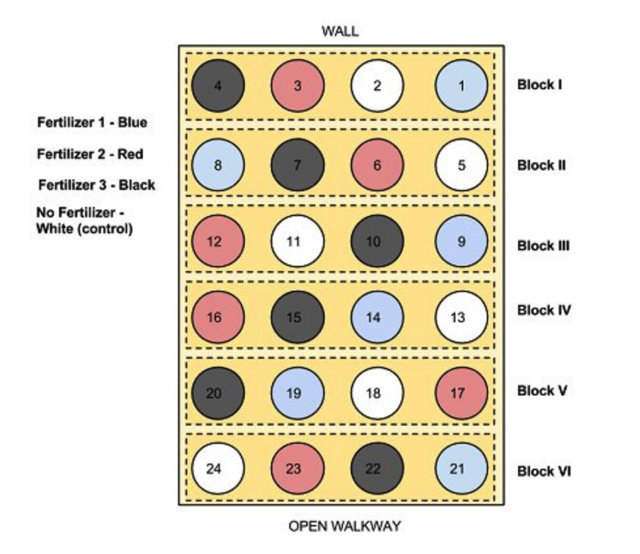
\includegraphics[width=8.89in]{images/BlockDesignGraphic}

The blocks are arranged along a gradient, say along the side of a hill, so represent low and high elevation and associated soil moisture. The blocks capture this background variation. THEN, each treatment level (1-4) is allocated a random position in each block.~~In the end, each treatment level is replicated across blocks (n = 6!). From: \url{https://www.researchgate.net/publication/322369242_Randomized_Block_Design_probiotic_example/figures?lo=1}

It is important to note that blocks exist at the time of the randomization of treatments to units. We cannot impose blocking structure on a completely randomized design after the fact; either the randomization was blocked or it was not.

We use an RCB to increase the power and precision of an experiment by decreasing the error variance. This decrease in error variance is achieved by finding groups of units that are homogeneous (blocks) and, in effect, repeating the experiment independently in the different blocks. The RCB is an effective design when there is a single source of extraneous variation in the responses that we can identify ahead of time and use to partition the units into blocks.

In short ALWAYS block your experiment, if you can.

You can have spatial blocks, or temporal blocks where you repeat the experiment at different times, or block by batch.

In general, any source of variation that you think may influence the response and which can be identified prior to the experiment is a candidate for blocking.

\hypertarget{an-example-of-the-rcbd}{%
\section{An example of the RCBD}\label{an-example-of-the-rcbd}}

Lets modify our previous example to including blocking. If you wish to replicate the analysis, the data are \texttt{plantYield\_Blocked.csv}. In these data, the means are similar to \texttt{plantYield} above, but Herbicide 1 is 10 units higher than the control and Herbicide 2 is 9 units higher. Furthermore, block 1 is supposed to be \textasciitilde10 units higher than blocks 2,3,4 while block 5 is \textasciitilde10 units lower.

\begin{verbatim}
##    plots block   treat      obs
## 1     11     1 Placebo 31.18707
## 2     12     1 Control 31.99603
## 3     13     1   Herb2 41.29937
## 4     14     1   Herb1 41.12746
## 5     21     2 Control 21.08111
## 6     22     2   Herb1 30.56917
## 7     23     2   Herb2 28.09290
## 8     24     2 Placebo 21.02990
## 9     31     3   Herb2 27.44097
## 10    32     3   Herb1 30.29749
\end{verbatim}

\hypertarget{analysing-the-crbd}{%
\section{Analysing the CRBD}\label{analysing-the-crbd}}

I'll leave it to you now to generate the following plot of the means ± standard errors from the \texttt{plantYield\_Blocked.csv} file.

This requires thinking hard about the use of dplyr tools (\texttt{group\_by()} and \texttt{summarise()}) and ggplot (adding more than one layer from two different sources of data - the summary data and the raw data). You need to make a \emph{sumDat} object for the means and se's. Then you need to plot the raw data, and overlay the mean±se info from the sumDat.

Can you see the variation between block 1 and 5? Block 2-4 are all similar\ldots. Block 1 is 10 units more, and Block 5 is 10 units less.

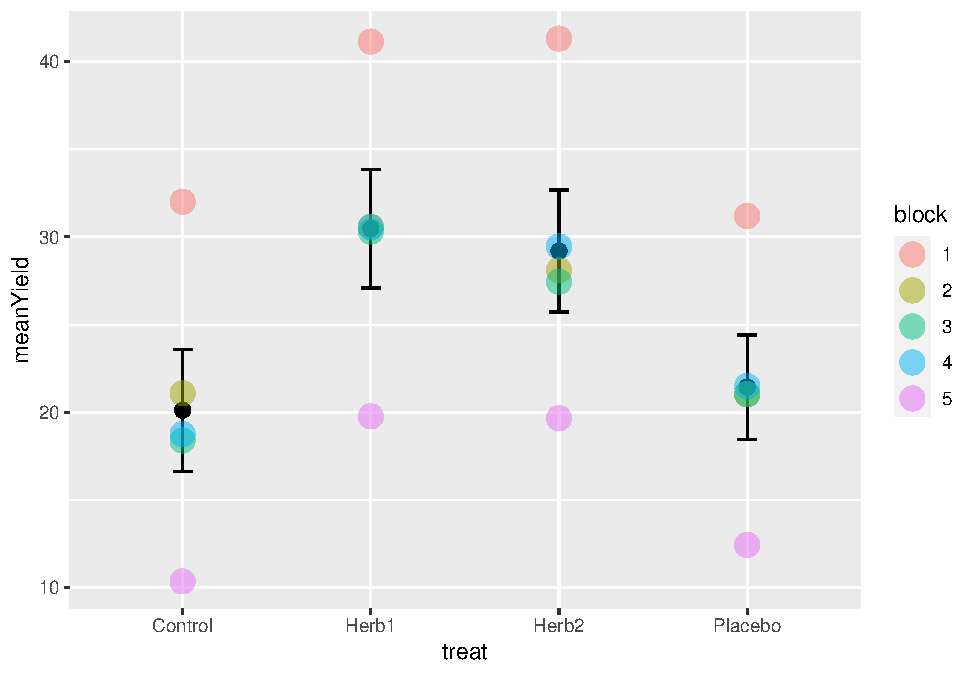
\includegraphics{Experimental-Design,-ANOVA-and-ANCOVA_files/figure-latex/unnamed-chunk-22-1.pdf}

\hypertarget{building-the-model}{%
\subsection{Building the model}\label{building-the-model}}

In order to understand what's going on with blocking, and it's importance, lets build two models. This is a good trick and a good process to learn. The first model is a \emph{naive} model that ignores block - treating this as a CRB. The second model is the \emph{correct} model, letting block absorb the variation we can see among the blocks 1, 2-4 and 5.

\begin{Shaded}
\begin{Highlighting}[]
\CommentTok{\# models}
\NormalTok{naive\_model }\OtherTok{\textless{}{-}} \FunctionTok{lm}\NormalTok{(obs }\SpecialCharTok{\textasciitilde{}}\NormalTok{ treat, plantYield\_Block)}
\CommentTok{\# note the order of these factors is important}
\CommentTok{\# put block first.... so we can absorb this variation first}
\CommentTok{\# the anova() table is a SEQUENTIAL table!}
\NormalTok{block\_model }\OtherTok{\textless{}{-}} \FunctionTok{lm}\NormalTok{(obs }\SpecialCharTok{\textasciitilde{}}\NormalTok{ block }\SpecialCharTok{+}\NormalTok{ treat, plantYield\_Block) }

\CommentTok{\# anova tables}
\FunctionTok{anova}\NormalTok{(naive\_model)}
\end{Highlighting}
\end{Shaded}

\begin{verbatim}
## Analysis of Variance Table
## 
## Response: obs
##           Df Sum Sq Mean Sq F value  Pr(>F)  
## treat      3 417.82 139.274  2.5085 0.09579 .
## Residuals 16 888.34  55.521                  
## ---
## Signif. codes:  0 '***' 0.001 '**' 0.01 '*' 0.05 '.' 0.1 ' ' 1
\end{verbatim}

\begin{Shaded}
\begin{Highlighting}[]
\FunctionTok{anova}\NormalTok{(block\_model)}
\end{Highlighting}
\end{Shaded}

\begin{verbatim}
## Analysis of Variance Table
## 
## Response: obs
##           Df Sum Sq Mean Sq F value    Pr(>F)    
## block      4 877.08 219.270  233.68 2.871e-11 ***
## treat      3 417.82 139.274  148.43 9.469e-10 ***
## Residuals 12  11.26   0.938                      
## ---
## Signif. codes:  0 '***' 0.001 '**' 0.01 '*' 0.05 '.' 0.1 ' ' 1
\end{verbatim}

The first important thing to focus on here is the difference in the Mean Sq Residual Errors - in the \texttt{naive\_model}, it is \(55.52\). In the \texttt{block\_model}, it is \(0.94\). Wow\ldots. a massive reduction in the residual error\ldots. where has it gone?

The second important thing to notice is that having allocated variation to block in the \texttt{block\_model}, and thus reducing the error variation, the \emph{treatment} effect shifts from being insignificant to significant. At this point you should try and recall how F-tests are generated (what is the equation!) to really understand how blocking has made such a different.

\hypertarget{are-the-estimates-of-the-parameters-what-we-expect}{%
\subsection{Are the estimates of the parameters what we expect?}\label{are-the-estimates-of-the-parameters-what-we-expect}}

Lets check that the model is estimating differences as we might have expected. We can do this using the summary table.

Let's remember that, for example, the mean of Herb1 is expected to be 10 units higher than control with a yield of 20, and block 1 is supposed to be \textasciitilde10 units higher than 2,3,4.

\begin{Shaded}
\begin{Highlighting}[]
\FunctionTok{summary}\NormalTok{(block\_model)}
\end{Highlighting}
\end{Shaded}

\begin{verbatim}
## 
## Call:
## lm(formula = obs ~ block + treat, data = plantYield_Block)
## 
## Residuals:
##     Min      1Q  Median      3Q     Max 
## -1.3505 -0.7196  0.2147  0.6396  1.0719 
## 
## Coefficients:
##              Estimate Std. Error t value Pr(>|t|)    
## (Intercept)   31.2184     0.6126  50.957 2.14e-15 ***
## block2       -11.2092     0.6850 -16.365 1.43e-09 ***
## block3       -12.1132     0.6850 -17.685 5.84e-10 ***
## block4       -11.3415     0.6850 -16.558 1.25e-09 ***
## block5       -20.8449     0.6850 -30.433 9.94e-13 ***
## treatHerb1    10.3450     0.6126  16.886 9.96e-10 ***
## treatHerb2     9.0721     0.6126  14.808 4.50e-09 ***
## treatPlacebo   1.3192     0.6126   2.153   0.0523 .  
## ---
## Signif. codes:  0 '***' 0.001 '**' 0.01 '*' 0.05 '.' 0.1 ' ' 1
## 
## Residual standard error: 0.9687 on 12 degrees of freedom
## Multiple R-squared:  0.9914, Adjusted R-squared:  0.9864 
## F-statistic: 197.1 on 7 and 12 DF,  p-value: 2.009e-11
\end{verbatim}

In this table, the \emph{INTERCEPT} is specifying the \textbf{FIRST BLOCK} and the \textbf{CONTROL TREATMENT LEVEL}. We know this because it's these words that are missing from the rest of the table, and they are each the first alpha-numerially in the list of blocks and treatments. Make sure you understand this. It's tricky, but once you get it, it becomes obvious\ldots. look for what is missing from the rest of the table!

\begin{itemize}
\tightlist
\item
  The value of the control, block 1 is approximately 30! Which is 20+10, which is what we expected.
\item
  The value of Herb1 is \textasciitilde10 units higher than this (remember, the value 9.84 is the DIFFERENCE between the control and treatment).
\item
  And the value of block 5 is reported as 20 unites lower than block 1 control. This too is correct because, as above, block 1 control is 10 units higher than the control mean (20+10) and block 5 is 10 units lower\ldots.
\end{itemize}

\emph{Make sure you get this logic!}

The take home message here is that these numbers from the model make complete sense with respect to the actual data. Furthermore, controlling for the among block variation \emph{gave us more power to detect a treatment effect}, something we would have missed had we not estimated the block source of variation.

\hypertarget{correct-standard-errors-for-a-figure}{%
\subsection{Correct Standard Errors for a Figure}\label{correct-standard-errors-for-a-figure}}

When we made our initial plot above, we calculated the standard error based on all observations among blocks. However, the variation we really wish to represent is the variation after having controlled for the blocking effects. This means that the standard deviation we should probably use is of the error variance from the correct model: \(0.94\). Can you see where this comes from? The \texttt{Mean\ Sq} column and \texttt{Residuals} row from the \texttt{anova()} table.

The standard deviation is the \(\sqrt{Var}\) and thus, our correct standard errors from the model are \(\sqrt{0.94}\)

\hypertarget{visreg---a-helpful-package-for-automating-this.}{%
\subsubsection{\texorpdfstring{\texttt{visreg} - a helpful package for automating this.}{visreg - a helpful package for automating this.}}\label{visreg---a-helpful-package-for-automating-this.}}

There is a very nice plotting function in the package \emph{visreg} that delivers these proper standard errors in a nice ggplot framework.

It presents points that are the partial residuals (deviation from the mean for each replicate), lines depicting the means, and shaded area as a 95\% confidence interval, calculated as \(1.96*SE\), where \emph{the SE is estimated from the model error variance} (just above). Compare this to your first graph.

\begin{Shaded}
\begin{Highlighting}[]
\FunctionTok{visreg}\NormalTok{(block\_model, }\StringTok{"treat"}\NormalTok{, }\AttributeTok{gg=}\ConstantTok{TRUE}\NormalTok{)}\SpecialCharTok{+}
  \FunctionTok{ylab}\NormalTok{(}\StringTok{"Yield"}\NormalTok{) }\SpecialCharTok{+} 
  \FunctionTok{xlab}\NormalTok{(}\StringTok{"Treatment"}\NormalTok{) }
\end{Highlighting}
\end{Shaded}

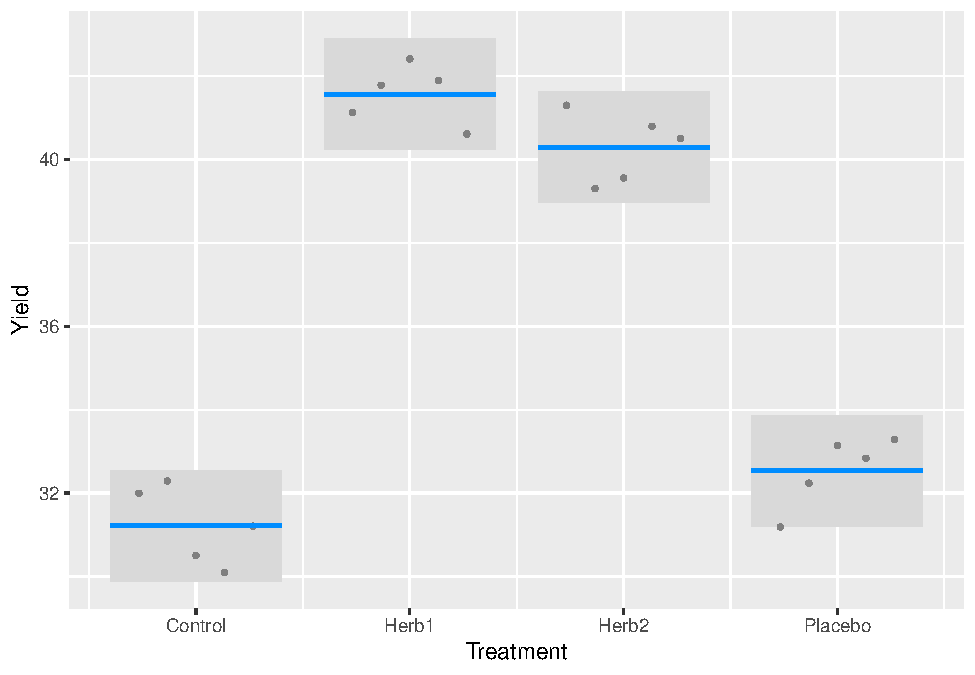
\includegraphics{Experimental-Design,-ANOVA-and-ANCOVA_files/figure-latex/unnamed-chunk-25-1.pdf}

\hypertarget{making-inference-in-a-blocked-model-confidence-intervals-and-contrasts}{%
\subsection{Making inference in a blocked model: confidence intervals and contrasts}\label{making-inference-in-a-blocked-model-confidence-intervals-and-contrasts}}

We are now in a very strong position to make inference.

Let's start with a rule of thumb linked to the 95\% confidence interval (CI). If the CIs in the figure above don't overlap, they are different; if they do, they are not. This indicates that Cont and Placebo are not significantly different (95\% confidence intervals overlap). Herb1 and Herb 2 are significantly different from these, but not each other.

This is OK. But it is not robust. Instead, let's revisit our \emph{post-hoc} and \emph{a priori} methods for evaluating differences among treatments. We can apply a tukey test and calculate all pairwise differences. This is not a good idea, but let's do it, using \emph{agricolae} and the \texttt{HSD.test()} function. Living large!

\begin{Shaded}
\begin{Highlighting}[]
\CommentTok{\# use agricolae HSD.test()}

\NormalTok{tukey\_out }\OtherTok{\textless{}{-}} \FunctionTok{HSD.test}\NormalTok{(block\_model, }\StringTok{"treat"}\NormalTok{, }\AttributeTok{group =} \ConstantTok{TRUE}\NormalTok{)}
\NormalTok{tukey\_out}\SpecialCharTok{$}\NormalTok{groups}
\end{Highlighting}
\end{Shaded}

\begin{verbatim}
##              obs groups
## Herb1   30.46167      a
## Herb2   29.18874      a
## Placebo 21.43581      b
## Control 20.11665      b
\end{verbatim}

This confirms our intuition and 95\% Confidence Interval insights. But is it correct?

Let's make a formal test, using the \texttt{contrast()} and \texttt{fit.contrast()} functions for of one of the pairwise tests that looks obvious - between Herb1 and Herb2. Even with block in the model, the second argument for \texttt{fit.contrast()} is the treatment for which the contrast is made.

\begin{Shaded}
\begin{Highlighting}[]
\CommentTok{\# fit.contrast from gmodels package}
\CommentTok{\# see that even with the block in the model}
\NormalTok{contrast }\OtherTok{\textless{}{-}} \FunctionTok{c}\NormalTok{(}\DecValTok{0}\NormalTok{,}\SpecialCharTok{{-}}\DecValTok{1}\NormalTok{,}\DecValTok{1}\NormalTok{,}\DecValTok{0}\NormalTok{)}
\FunctionTok{fit.contrast}\NormalTok{(block\_model, }\StringTok{"treat"}\NormalTok{, contrast)}
\end{Highlighting}
\end{Shaded}

\begin{verbatim}
##                       Estimate Std. Error   t value   Pr(>|t|)
## treat c=( 0 -1 1 0 ) -1.272934  0.6126423 -2.077777 0.05985811
## attr(,"class")
## [1] "fit_contrast"
\end{verbatim}

Amazing. The contrast defining a specific test provides a different answer than the post-hoc Tukey test. This is important\ldots{} the Tukey Test makes lots of tests and they are penalised for so many tests. But, the contrast is the correct and most reliable result. While both \emph{fit.contrast} and \emph{HSD.test} both manage the model complexity and variance estimates properly, only the contrast reduces the probability of finding a significant difference by chance or failing to find one.

\hypertarget{designs-for-testing-for-interactions-the-two-way-anova-and-factorial-designs.}{%
\chapter{Designs for testing for interactions: the two-way ANOVA and factorial designs.}\label{designs-for-testing-for-interactions-the-two-way-anova-and-factorial-designs.}}

\hypertarget{introducing-interactions}{%
\section{Introducing Interactions}\label{introducing-interactions}}

In the previous sections, and the 1-way ANOVA module in week 7, we have focused on a single explanatory variable. In week 7, it was the \texttt{parasite} factor. In the previous chapters focusing on yield, it was the \texttt{herbicide} treatment. In these cases, the question we are asking is about a single, main effect. However, there are many cases where we design experiments that might have two variables. For example, we may be interesting in the effect of \texttt{parasite} on growth but also whether this effect varies by the amount of food available. Or we might be interested in the yeild of a crop as a function of the herbicide, but also of soil water content. Or we might be interested in the rate of cell division as a function of a growth hormon, but also of whether this varies by the presence of a calcium blocker. In all of these cases we are asking a question about whether the effect of one treatment varies by the level of another. Thus, our question here is about an \emph{interaction}.

Before jumping into an example, let's introduce a simple statement that forms the core of both asking and interpreting \emph{interactions}.

If there is an interaction between two explanatory variables, X and Z, on our response variable Y, then:

\begin{quote}
The effect of X on Y varies by Z. \textbf{OR} The effect of X on Y depends on Z.
\end{quote}

This use of \emph{varies by} \textbf{OR} \emph{depends on} defines context dependency and that's what defines interactions.

\hypertarget{an-example-with-co2-and-uv-b-solar-radiation-impact-on-plant-growth-in-the-artic.}{%
\subsection{An Example with CO2 and UV-B solar radiation impact on plant growth in the artic.}\label{an-example-with-co2-and-uv-b-solar-radiation-impact-on-plant-growth-in-the-artic.}}

Context: an arctic tundra study
Increasing ultraviolet-B (+UV-B) radiation from ozone depletion (the arctic ozone hole)
Increasing atmospheric CO2 (+CO2) from anthropogenic emissions
For plants: UV-B potentially harmful, +CO2 potentially beneficial
Therefore +CO2 could alleviate UV-B damage impacts.

\emph{Hypothesis}

The effect of UV-B radiation on growth will depend on levels of CO2

\emph{Predictions}:

+UV-B radiation will reduce the growth of arctic plants
+CO2 will increase the growth of arctic plants
+UV-B radiation impacts will be less under +CO2

What is unique about this context, hypothesis, and predictions?

It's the presentation of CO2 and UVB in the same statement and the use of words like ``the effect of X will alleviate the impacts of Y'' and words like ``the effects of X will be less under Y''. These words and phrases reflect the \emph{context dependency} of the effects of treatment levels.

Thus, to restate what we introduced above\ldots. when we talk about \emph{interactions}, we can rely on a very simple vocabulary that is independent of the actual treatment levels: we can always describe an interaction like this:

\begin{quote}
The effect of X on Y depends on Z.
\end{quote}

or

\begin{quote}
The effect of X on Y varies by Z.
\end{quote}

In this `rubric', Y is the response variable, and X and Z are explanatory, independent variables. So, in our example above,

\begin{quote}
the effect of CO2 on plant biomass yield depends on UV-B radiation levels.
\end{quote}

OR

\begin{quote}
the effect of CO2 on plant biomass yield varies with UV-B radiation levels.
\end{quote}

This simple phrasing describes any interaction.

\hypertarget{numerical-example-for-emphasis}{%
\subsubsection{Numerical example for emphasis}\label{numerical-example-for-emphasis}}

Let's imagine the following situation. The folowing three numbers are what we call \emph{Main Effects}:

Control = 20g Yield
UV-B = 10g Yield
C02 = 29g Yield

These numbers allow us to calculate the \emph{Additive Effect}, where the effect of both CO2 and UV-B is simply estimated by adding the two independent effects together:

ADDITIVE RESULT: C02 + UV-B = 39g Yield

However, this additive outcome may not be what happens. Imagine if there were Synergy - the effects are more than the sum of the independent effects - or Antagonism - the effects are less than expected because one offsets the other.

SYNERGISTIC RESULT: C02 + UV-B = 60g Yield
ANTAGONISTIC RESULT: C02 + UV-B = 19g Yield

\hypertarget{the-factorial-design-why-study-interactions}{%
\subsubsection{The Factorial Design: Why Study Interactions?}\label{the-factorial-design-why-study-interactions}}

The UV-B and C02 experiment could be thought of as two experiments -- a Control vs UV-B and a Control vs C02 experiment. If we combine these we get a Factorial Experiment where we can actually estimate whether there is an interaction, and whether it is synergy or antagonism. In the factorial design for this example, there are four treatment levels and all combinations of all treatments.

\begin{itemize}
\tightlist
\item
  Control
\item
  UV-B
\item
  C02
\item
  UV-B + C02
\end{itemize}

Some of you may be thinking that we could simply treat each of these treatment levels indepdently, as unique treatments levels - e.g.~the one-way ANOVA. But we don't. We design and analyse the data we collect in a two-way analysis - a factorial design. Two-way ANOVA is the design

Factorial treatments have two main advantages over the 1-way approach.

When factors \emph{DO interact} -- so the effect of C02 depends on UV-B -- then we can estimate the interaction - the dependency. \emph{One-way designs} cannot do this, and can lead to serious misunderstandings (because we are assuming that the effect of one thing DOES NOT depend on the other).

Furthermore, when factors \emph{DON'T interact}, \emph{factorial designs} are more precise (smaller error variance) at estimating the main (non-interacting effects) than one-way designs experiments.

Hence ALWAYS use factorial designs when your experimental design contains the interaction (when you are asking the question that includes the word(s) \emph{depends} or \emph{varies by}!

\hypertarget{a-factorial-design-and-the-two-way-anova}{%
\section{A Factorial Design and the Two-Way ANOVA}\label{a-factorial-design-and-the-two-way-anova}}

The following dataset \texttt{plantYield\_factorial} contains two observation columns - \texttt{yield\_ind} are data where there is NO INTERACTION. \texttt{yield\_int} are data where there are an interaction. We will use both of these to showcase how to work the 2-way ANOVA and the analysis of a factorial design.

We note that these data have replication and randomisation. There are \emph{four} replicate plants/plots allocated randomly to each of the four treatment combinations.

Here is the evidence of the factorial design

\begin{Shaded}
\begin{Highlighting}[]
\FunctionTok{xtabs}\NormalTok{(}\SpecialCharTok{\textasciitilde{}}\NormalTok{UVB}\SpecialCharTok{+}\NormalTok{CO2, }\AttributeTok{data =}\NormalTok{ plantYield\_factorial)}
\end{Highlighting}
\end{Shaded}

\begin{verbatim}
##       CO2
## UVB    Con CO2+
##   Con    4    4
##   UVB+   4    4
\end{verbatim}

\hypertarget{plot-the-factorial-design}{%
\subsection{Plot the factorial design!}\label{plot-the-factorial-design}}

Here we combine some dplyr magic (calculating means in each group - there are two grouping variables!), some ggplot magic (adding the lines connecting the means on top of the raw data) and the beauty of patchwork, the package for plot layouts.

Our goal here is to plot the data that does not have the interaction next to a plot of the data that does have the interaction.

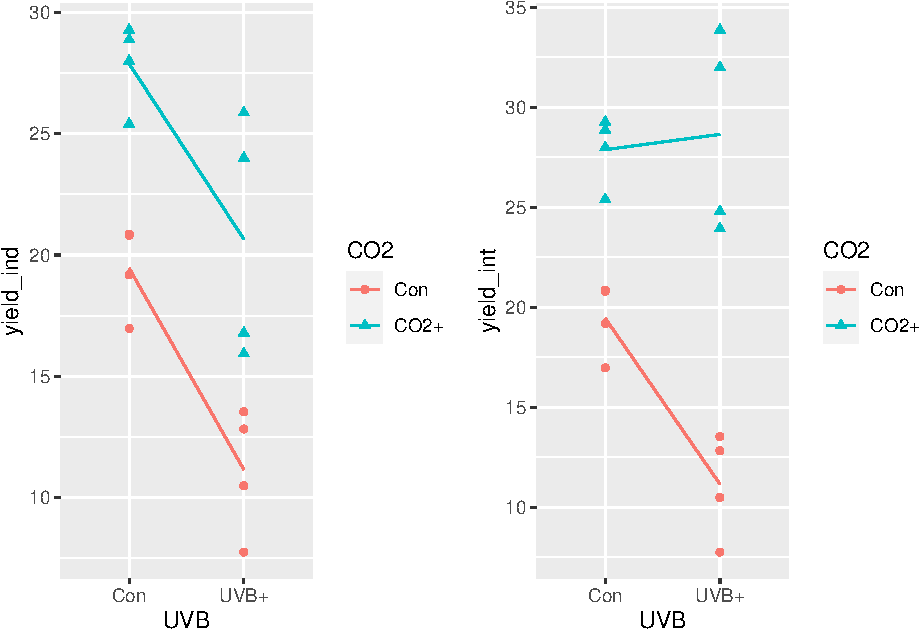
\includegraphics{Experimental-Design,-ANOVA-and-ANCOVA_files/figure-latex/unnamed-chunk-31-1.pdf}

Given what you've read above, you should be able to fill in these blanks:

What you see above on the left, is a pattern that suggest that the effect of \_\_\_\_\_\_ on \_\_\_\_\_\_\_\_ does not vary by \_\_\_\_\_\_\_\_.

In contrast, on the right the pattern suggests that the effect of \_\_\_\_\_\_ on \_\_\_\_\_\_\_\_ \_\_\_\_\_\_\_\_ by \_\_\_\_\_\_\_\_:

\hypertarget{how-to-analyse-and-interpret-the-factorial-design}{%
\subsection{How to analyse and interpret the factorial design}\label{how-to-analyse-and-interpret-the-factorial-design}}

As with the plotting, we now analyse each data set.

We also make a mistake of analysing the data that has an interaction with a model that does not specify this interaction.

We are thus making three models. A model of the no interaction data without specifying and interaction, a model of the interaction data without specifying and interaction and a model of the interaction data with and interaction specified. This second model is incorrect, but fitting it helps illuminate why you should fit the interaction if your design contains the potential for an interaction (a factorial design).

\begin{quote}
An Important Note on what + and * mean in models. In the below model specification, you will see CO2 + UVB and CO2 * UVB. Using the vocabulary from above, CO2 + UVB is specifying independent additive effects. In the ANOVA table produced by anova(), there will be three lines: one for CO2, one for UVB and one for residuals. In contrast, CO2 * UVB produces four lines of output in the ANOVA table. We say that CO2 * UVB expands to include the main, independent effects of CO2 and UVB, but also the interaction between them. So CO2 * UVB == CO2 + UVB + CO2:UVB where the last term is the interaction. Thus, there are four lines reported: one for CO2, one for UVB, one for the interaction and one for residuals.
\end{quote}

\begin{Shaded}
\begin{Highlighting}[]
\CommentTok{\# A Correct model with no interaction on data with no interaction}
\NormalTok{int\_mod\_1 }\OtherTok{\textless{}{-}} \FunctionTok{lm}\NormalTok{(yield\_ind }\SpecialCharTok{\textasciitilde{}}\NormalTok{ CO2 }\SpecialCharTok{+}\NormalTok{ UVB, }\AttributeTok{data =}\NormalTok{ plantYield\_factorial)}

\CommentTok{\# A Correct model with interaction where the should be an interaction}
\NormalTok{int\_mod\_2 }\OtherTok{\textless{}{-}} \FunctionTok{lm}\NormalTok{(yield\_int }\SpecialCharTok{\textasciitilde{}}\NormalTok{ CO2 }\SpecialCharTok{*}\NormalTok{ UVB, }\AttributeTok{data =}\NormalTok{ plantYield\_factorial)}

\CommentTok{\# THE WRONG MODEL: model without interaction, on data that should use the interaction}
\NormalTok{int\_mod\_3 }\OtherTok{\textless{}{-}} \FunctionTok{lm}\NormalTok{(yield\_int }\SpecialCharTok{\textasciitilde{}}\NormalTok{ CO2 }\SpecialCharTok{+}\NormalTok{ UVB, }\AttributeTok{data =}\NormalTok{ plantYield\_factorial)}

\FunctionTok{anova}\NormalTok{(int\_mod\_1) }\CommentTok{\# Good model, no interaction in the data and none in the model}
\end{Highlighting}
\end{Shaded}

\begin{verbatim}
## Analysis of Variance Table
## 
## Response: yield_ind
##           Df Sum Sq Mean Sq F value    Pr(>F)    
## CO2        1 321.00  321.00  35.905 4.504e-05 ***
## UVB        1 241.27  241.27  26.987 0.0001726 ***
## Residuals 13 116.22    8.94                      
## ---
## Signif. codes:  0 '***' 0.001 '**' 0.01 '*' 0.05 '.' 0.1 ' ' 1
\end{verbatim}

\begin{Shaded}
\begin{Highlighting}[]
\FunctionTok{anova}\NormalTok{(int\_mod\_2) }\CommentTok{\# Good model, interaction in the data and interaction in the model}
\end{Highlighting}
\end{Shaded}

\begin{verbatim}
## Analysis of Variance Table
## 
## Response: yield_int
##           Df Sum Sq Mean Sq F value    Pr(>F)    
## CO2        1 671.67  671.67 70.0311 2.364e-06 ***
## UVB        1  56.75   56.75  5.9165   0.03159 *  
## CO2:UVB    1  82.15   82.15  8.5654   0.01268 *  
## Residuals 12 115.09    9.59                      
## ---
## Signif. codes:  0 '***' 0.001 '**' 0.01 '*' 0.05 '.' 0.1 ' ' 1
\end{verbatim}

\begin{Shaded}
\begin{Highlighting}[]
\FunctionTok{anova}\NormalTok{(int\_mod\_3) }\CommentTok{\# Bad model, interaction in the data, but failure to specify in the model}
\end{Highlighting}
\end{Shaded}

\begin{verbatim}
## Analysis of Variance Table
## 
## Response: yield_int
##           Df Sum Sq Mean Sq F value   Pr(>F)    
## CO2        1 671.67  671.67  44.269 1.58e-05 ***
## UVB        1  56.75   56.75   3.740  0.07519 .  
## Residuals 13 197.24   15.17                     
## ---
## Signif. codes:  0 '***' 0.001 '**' 0.01 '*' 0.05 '.' 0.1 ' ' 1
\end{verbatim}

Let's focus on model 2 and how we interpret this. The ANOVA table now has multiple rows. We saw this before with the block design. The important thing to note here is that the table is now read \emph{sequentially}. We first note that CO2 explains \(507.19\) units of variation (Mean Sq) in plant Yield. Having captured this variation, we then note that UVB captures \(216.29\) additional units. Then, having capture the variation caused directly by CO2 and UVB, we now see that the interaction - asking whether the effect of CO2 varies by UVB - explains an additional \(127.72\) units. And\ldots{} there are \(11.11\) units of unexplained variation.

Great. So, remember as well how we calculate the F-value. In the ANOVA (categorial variable) framework, the F-value is the ratio of variance explained by the factor relative to the residual variation. So that's where the F values come from\ldots. And recall that BIG F-values indicate that more variation is allocated to the treatment levels, versus what's left over. The bigger the numerator value relative to the residual denominator, the more variation this term has explained.

In this experimental design, and any like it, one must remember that there is actually a single question, and it does not related to the independent main effects.It relates only to the interaction term: we designed this experiment to test the hypothesis that the effect of CO2 on yield varies by UVB. There is only a single choice of answer - yes or no. In this case, having captured variation with each independent effect, there is still a large amount of variation captured by `allowing' the effects of each to vary by the other. Under a null hypothesis that these two variables to not interact (do not depend on each other), getting a Mean square estimate of \(127.72\) relative to the residual of \(11.11\) is very unlikely. So we reject the null!

Spend some time investigating what has happened with model 2 and model 3 and recall that ONLY ONE OF THEM IS CORRECT, regardless of whether the data look like the left or right panel above. Note the differences in the outputs. Note what we infer if we model the interaction data incorrectly.

There is no free lunch.

You must understand your data and your question and you must fit the model that correctly matches your design! In this case, there really is only one model you should fit. It is model 2. EVEN if the data look like the left panel, with no interaction, this experiment was designed to test the hypothesis that the effect of CO2 varies by UVB. You can only accept or reject the null hypothesis of no interaction by fitting model 2. You can not guess the right model from the picture. The design dictates the model. But, you can guess the answer\ldots.

\hypertarget{visreg-and-the-2-way-anova}{%
\subsection{visreg and the 2-way ANOVA}\label{visreg-and-the-2-way-anova}}

Don't forget that the correct standard error for the `result' is the residuals mean squared. You can use the dplyr + ggplot2 method, or visreg to estimate these. Here we use the \texttt{visreg} package and put the figure next to our original ggplot for the interaction data. Either of these would be OK for presentation, and most would opt for the left panel. Note the use of the the correct model for the design and question (model 2).

\begin{Shaded}
\begin{Highlighting}[]
\NormalTok{p3 }\OtherTok{\textless{}{-}} \FunctionTok{visreg}\NormalTok{(int\_mod\_2,}\StringTok{"CO2"}\NormalTok{,}\AttributeTok{by=}\StringTok{"UVB"}\NormalTok{, }\AttributeTok{gg=}\ConstantTok{TRUE}\NormalTok{) }\SpecialCharTok{+}
  \FunctionTok{theme\_classic}\NormalTok{()}

\NormalTok{p2}\SpecialCharTok{+}\NormalTok{p3}
\end{Highlighting}
\end{Shaded}

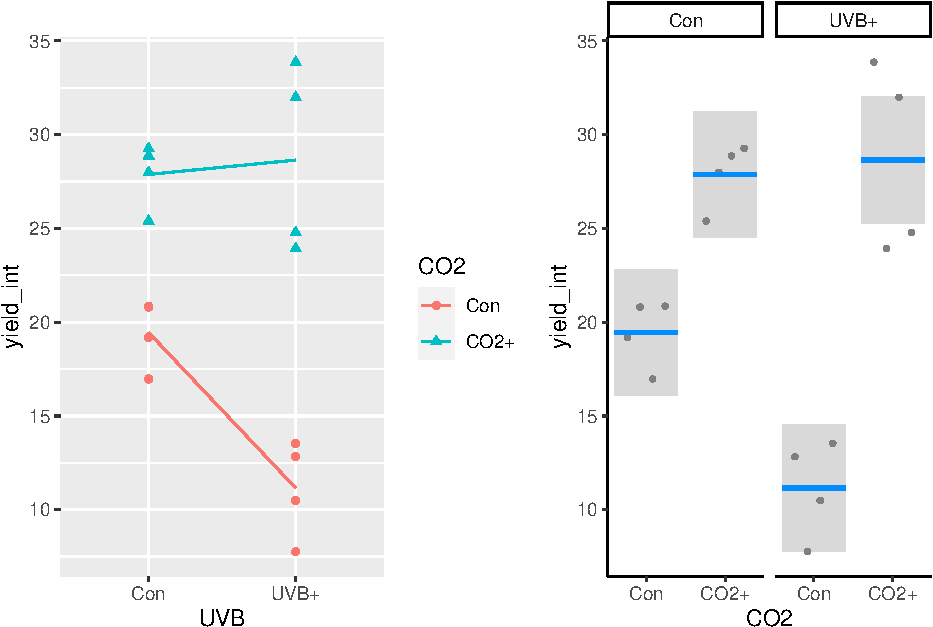
\includegraphics{Experimental-Design,-ANOVA-and-ANCOVA_files/figure-latex/unnamed-chunk-33-1.pdf}

\hypertarget{interactions-part-2-introducing-the-ancova-analysis-of-covariance}{%
\chapter{Interactions Part 2: Introducing the ANCOVA (analysis of covariance)}\label{interactions-part-2-introducing-the-ancova-analysis-of-covariance}}

In the previous chapters, we introduced classic experimental design principles, and in doing so, we focused on revisiting the 1-way ANOVA and introduced the 2-way ANOVA. In these models, the explanatory variables are categorical (they are factors). This means explanatory variable has distinct, discrete categories or \emph{levels}.

In many of our experiments, however, we might combine a categorical variable with a continuous variable. For example, we might estimate eggs produced as a function of body size (continuous) and season (categorical). Or we might estimate the effect of a mutagen (continuous) on tumour formation in wild type vs.~genetically modified (categorical) fruit flies.

These simple examples describe an ANCOVA, where the one explanatory variable is continuous (e.g.~body size or mutagen) and the other is categorical (e.g.~season or fly-type). When this is the case, we are essentially combining the ANOVA with the Regression model! If we recall that regression is largely about estimating slopes and intercepts, we might think, hey, COOL, so in an ANCOVA, we can ask if the categorical variable alters the slope or not\ldots.. and that'd be correct.

What is very important to understand is that our core statement about interactions does not change.

\begin{quote}
The effect of X on Y varies by Z, translates to a) The effect of body size on egg production varies by season; or b) the effect of mutagen on tumour formation varies by fly-type.
\end{quote}

When written like this, the previous statements about slopes should be even more clear. The effect of body size (continuous) on egg production is a regression and we estimate a slope. The effect of the mutagen concentration on tumour formation is a regression and we estimate a slope. We then can ask whether this slope is different between seasons or fly-type.

\hypertarget{what-this-chapter-covers.}{%
\section{What this chapter covers.}\label{what-this-chapter-covers.}}

This chapter will focus on the ANCOVA, but it also touches on additional concepts. The primary foci are thus:

\begin{enumerate}
\def\labelenumi{\arabic{enumi}.}
\tightlist
\item
  The ANCOVA model
\item
  transformations
\item
  plotting model results when you've made transformations.
\end{enumerate}

\hypertarget{setting-up-the-various-ideas.}{%
\section{Setting up the various ideas.}\label{setting-up-the-various-ideas.}}

Let's start by looking at an example where the effect of Height on Weight varies by Sex. This is a classic set of data from numerous organisms\ldots. it captures biologically the question about sexual dimorphism - does the relationship between Height and Weight (a regression with the continuous variable Weight) vary by Sex (the categorical variable {[}e.g.~ANOVA{]}, in this case M/F but it can be more depending on organism)?

This relationship can take on many patterns.

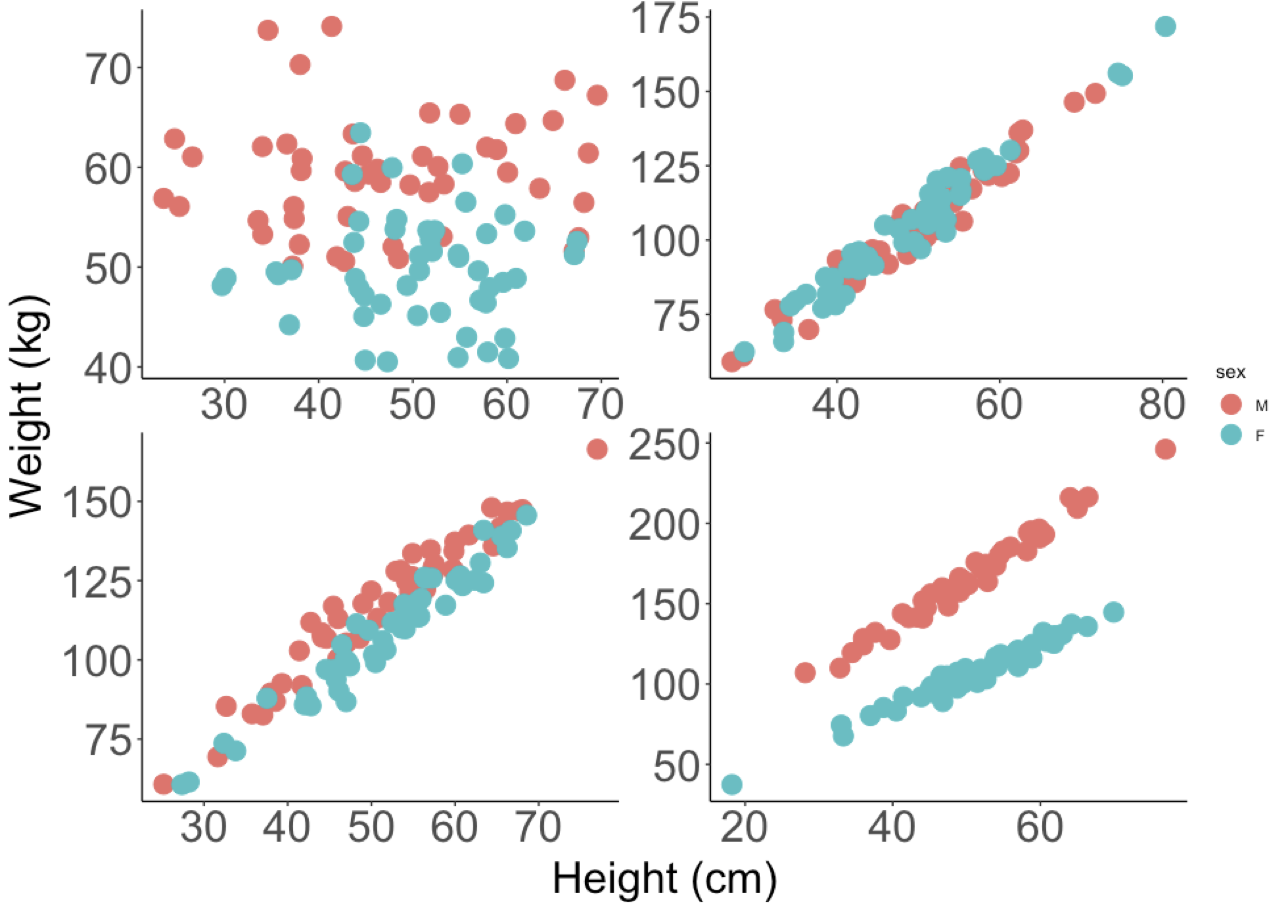
\includegraphics[width=17.89in]{images/ANCOVA_1}

\begin{itemize}
\tightlist
\item
  In the upper left we see a pattern where Males are heavier than Females, but there is no effect of Height on Weight.
\item
  In the upper right, we see that there is a positive relationship between Weight and Height, but no differences between Males and Females.
\item
  In the lower left, we might argue that there is a positive relationship between Weight and Height, that the relationship between Weight and Height does not vary (the slope is the same) and that Males are heavier (the red dots are mostly above the blue)
\item
  In the lower right, we see evidence of an interaction - the effect of Height on Weight (the slopes), varies by Sex.
\end{itemize}

It's quite important to recognise that each of these patterns (predictions) is possible outcome to testing the SAME null hypothesis. The key thing to remember is that we have an \emph{a priori} (in advance hypothesis) that there is no difference between the slopes for males and females. Regardless of the pattern, we should specify the appropriate model to test your the hypothesis and answer the question that motivated the design of the experiment and data collection.

Let's be super clear: in these data we start with the fundamental question that uses the same vocabulary that we used in the previous chapter - does the effect of Height on Weight vary by Sex. The data might look like any one of the above patterns. BUT, there is only one model syntax in the above figure that tests the null hypothesis and gives us a chance to evaluate the predictions: \texttt{lm(Weight\ \textasciitilde{}\ Height\ *\ Sex,\ data\ =\ data.frame.name)}.

\begin{quote}
If you need a refresher on what the * symbol means, pop back to chapter 5 where we explain this when we fit the models; we also review this below.
\end{quote}

\hypertarget{anticipating-the-anova-table-for-an-ancova-model}{%
\subsection{Anticipating the ANOVA table for an ANCOVA model}\label{anticipating-the-anova-table-for-an-ancova-model}}

Let us also recall the sequential nature of the ANOVA table output. This is about what we expect to see, having fit a model, which we will do below. In contrast to the ANOVA, with an ANCOVA, we will see first an estimate of variation explained by the continuous variable, then the categorical variable and finally, after seeing the report on both of those, an estimate of the variation attributable to the interaction. Another way to think of this is as follows (explore the figures above along with this):

What is the estimate of the intercept and slope, ignoring the different categories, and how much variation does this explain.
What happens if we let there be two lines, one for each category, but with the same slope (e.g.~different intercepts, but same slope). Does this explain more variation?
Finally, what if we let there be two lines, and different slopes (the interaction exists) - does this explain additional variation?

If we get to the last scenario, and the answer is yes, after all the other options, the \emph{different slopes} does capture variation in our response, we have evidence of an interaction.

\hypertarget{working-through-an-ancova-example.}{%
\section{Working through an ANCOVA example.}\label{working-through-an-ancova-example.}}

Let's work with a built in dataset in R - the Davis Study, which is exactly these data. The associated assignment is another example.

The process of doing this will follow a tried and true approach to analysing data. You should have this workflow fully embedded in your head now:

\begin{enumerate}
\def\labelenumi{\arabic{enumi})}
\tightlist
\item
  PLOT the Data
\item
  Build the model to test the hypothesis
\item
  Check the Assumptions
\item
  Make Inference
\item
  Update the Figure for Publication
\end{enumerate}

\hypertarget{organise-the-packages-and-get-the-data-and-make-your-picture}{%
\subsection{Organise the packages and get the data and make your picture}\label{organise-the-packages-and-get-the-data-and-make-your-picture}}

The data we are using is an example dataset built into R, but embedded in the \texttt{carData} package, which is installed with the \texttt{car} package - download and install this and they you can use the following code (don't forget the \texttt{tidyverse}, \texttt{agricolae}, \texttt{ggfortify}, \texttt{visreg} etc).

\begin{quote}
These data ARE NOT on the blackboard site.
\end{quote}

Note also that if you are building your own script, you need the following packages: \texttt{tidyverse}, \texttt{ggfortify}, \texttt{visreg}, \texttt{patchwork}

\begin{Shaded}
\begin{Highlighting}[]
\FunctionTok{library}\NormalTok{(tidyverse)}
\FunctionTok{library}\NormalTok{(ggfortify)}
\FunctionTok{library}\NormalTok{(visreg)}
\FunctionTok{library}\NormalTok{(patchwork)}

\CommentTok{\# this creates a working version of the davis data for you.}
\CommentTok{\# the carData:: syntax is a way to use this package without using}
\CommentTok{\# the library() function.}
\NormalTok{Davis }\OtherTok{\textless{}{-}}\NormalTok{ carData}\SpecialCharTok{::}\NormalTok{Davis}

\CommentTok{\# check it out}
\FunctionTok{glimpse}\NormalTok{(Davis)}
\end{Highlighting}
\end{Shaded}

\begin{verbatim}
## Rows: 200
## Columns: 5
## $ sex    <fct> M, F, F, M, F, M, M, M, M, M, M, F, F, F, F, F, M, F, M, F, M, ~
## $ weight <int> 77, 58, 53, 68, 59, 76, 76, 69, 71, 65, 70, 166, 51, 64, 52, 65~
## $ height <int> 182, 161, 161, 177, 157, 170, 167, 186, 178, 171, 175, 57, 161,~
## $ repwt  <int> 77, 51, 54, 70, 59, 76, 77, 73, 71, 64, 75, 56, 52, 64, 57, 66,~
## $ repht  <int> 180, 159, 158, 175, 155, 165, 165, 180, 175, 170, 174, 163, 158~
\end{verbatim}

\begin{Shaded}
\begin{Highlighting}[]
\CommentTok{\# make the most basic of exploratory plots.}
\FunctionTok{ggplot}\NormalTok{(Davis, }\FunctionTok{aes}\NormalTok{(}\AttributeTok{x =}\NormalTok{ height, }\AttributeTok{y =}\NormalTok{ weight, }\AttributeTok{col =}\NormalTok{ sex))}\SpecialCharTok{+}
  \FunctionTok{geom\_point}\NormalTok{()}
\end{Highlighting}
\end{Shaded}

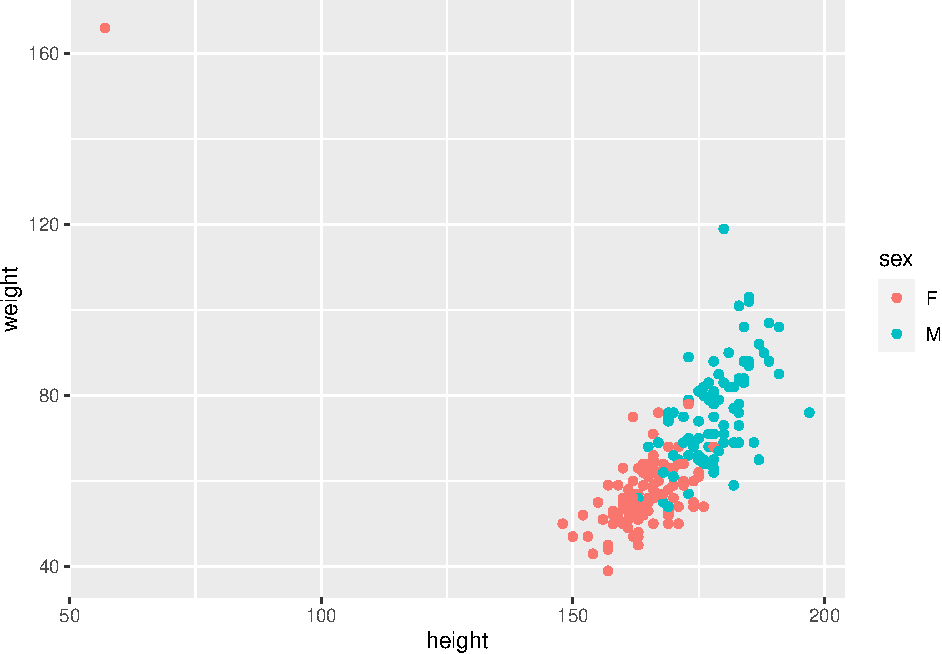
\includegraphics{Experimental-Design,-ANOVA-and-ANCOVA_files/figure-latex/unnamed-chunk-36-1.pdf}

Whoa!\ldots{} what's going on here? Well,here is a massive justification of why we say \emph{``always plot your data''} before you do anything. It looks like one of the data points has the height and weight data entered incorrectly, the wrong way around. This is a `feature' of this dataset. Of course you could go back to your master spreadsheet and make the corretion, which is a good idea in real life, but let's see how to fix this using R. Let's fix that. Lets find the row with the mistake by looking for height values \textless100, and then make the switch.

\begin{Shaded}
\begin{Highlighting}[]
\CommentTok{\#which row? 12}
\NormalTok{Davis }\SpecialCharTok{\%\textgreater{}\%} \FunctionTok{filter}\NormalTok{(height }\SpecialCharTok{\textless{}} \DecValTok{100}\NormalTok{)}
\end{Highlighting}
\end{Shaded}

\begin{verbatim}
##    sex weight height repwt repht
## 12   F    166     57    56   163
\end{verbatim}

\begin{Shaded}
\begin{Highlighting}[]
\CommentTok{\# BASE R syntax to see each observation}
\NormalTok{Davis}\SpecialCharTok{$}\NormalTok{weight[}\DecValTok{12}\NormalTok{]}
\end{Highlighting}
\end{Shaded}

\begin{verbatim}
## [1] 166
\end{verbatim}

\begin{Shaded}
\begin{Highlighting}[]
\NormalTok{Davis}\SpecialCharTok{$}\NormalTok{height[}\DecValTok{12}\NormalTok{]}
\end{Highlighting}
\end{Shaded}

\begin{verbatim}
## [1] 57
\end{verbatim}

\begin{Shaded}
\begin{Highlighting}[]
\CommentTok{\# BASE R syntax to change the specific values in the specific row}
\NormalTok{Davis}\SpecialCharTok{$}\NormalTok{weight[}\DecValTok{12}\NormalTok{] }\OtherTok{\textless{}{-}} \DecValTok{57}
\NormalTok{Davis}\SpecialCharTok{$}\NormalTok{height[}\DecValTok{12}\NormalTok{] }\OtherTok{\textless{}{-}} \DecValTok{166}

\CommentTok{\# replot}
\FunctionTok{ggplot}\NormalTok{(Davis, }\FunctionTok{aes}\NormalTok{(}\AttributeTok{x =}\NormalTok{ height, }\AttributeTok{y =}\NormalTok{ weight, }\AttributeTok{col =}\NormalTok{ sex))}\SpecialCharTok{+}
  \FunctionTok{geom\_point}\NormalTok{()}
\end{Highlighting}
\end{Shaded}

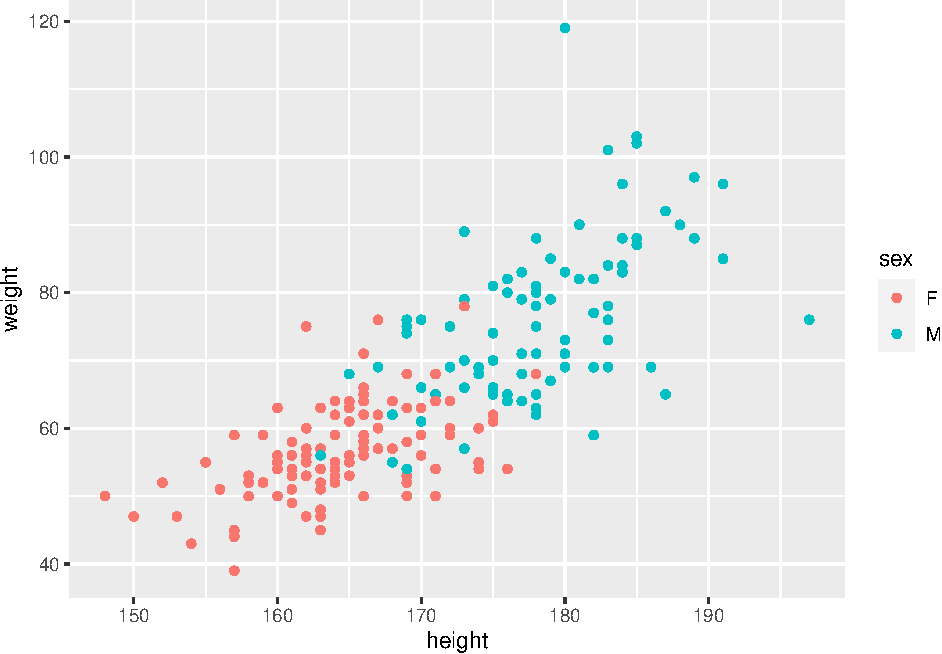
\includegraphics{Experimental-Design,-ANOVA-and-ANCOVA_files/figure-latex/unnamed-chunk-37-1.pdf}

Excellent. Let's look at this picture and ask ourselves the null hypothesis question: does the effect of Height on Weight vary by Sex? What do you think?

We can actually get a bit of help here. We can use some ggplot magic to help us make this GUESS. Let's use \texttt{geom\_smooth()} to help us guess the answer.

\begin{quote}
NOTE: this is not doing statistics. This is using graphics to help guide insight and our expectation of the outcome before doing the statistical test of our hypothesis.
\end{quote}

\begin{Shaded}
\begin{Highlighting}[]
\FunctionTok{ggplot}\NormalTok{(Davis, }\FunctionTok{aes}\NormalTok{(}\AttributeTok{x =}\NormalTok{ height, }\AttributeTok{y =}\NormalTok{ weight, }\AttributeTok{col =}\NormalTok{ sex))}\SpecialCharTok{+}
  \FunctionTok{geom\_point}\NormalTok{()}\SpecialCharTok{+}
  \CommentTok{\# add a best fit line to each group (the sex category)}
  \FunctionTok{geom\_smooth}\NormalTok{(}\AttributeTok{method =}\NormalTok{ lm, }\AttributeTok{se =} \ConstantTok{FALSE}\NormalTok{)}
\end{Highlighting}
\end{Shaded}

\begin{verbatim}
## `geom_smooth()` using formula 'y ~ x'
\end{verbatim}

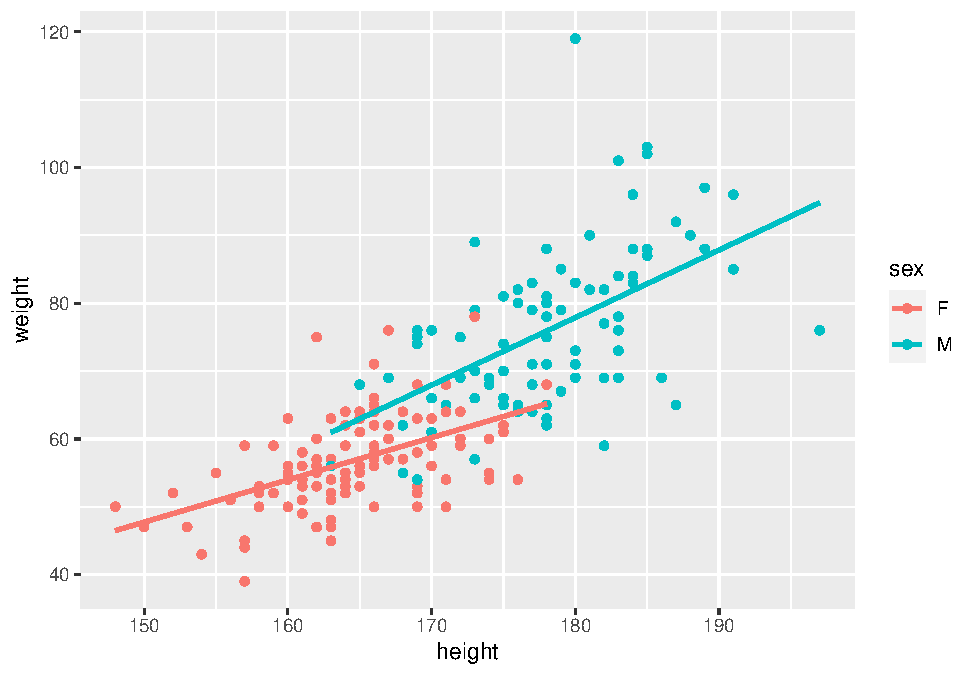
\includegraphics{Experimental-Design,-ANOVA-and-ANCOVA_files/figure-latex/unnamed-chunk-38-1.pdf}

Again, we have not `proven' anything or tested our hypothesis. What we have is a good guess though. We can guess that

\begin{enumerate}
\def\labelenumi{\arabic{enumi}.}
\tightlist
\item
  Males are heavier than females (what is the difference in the intercepts?)
\item
  The effect of height on weight is positive (the slope(s) are positive, not negative)
\item
  There \emph{might} be a difference in slopes - the Male line looks steeper.
\end{enumerate}

We might even go as far to estimate by eye the overall slope, assuming that there is no effect of Sex. Recalling that the slope is the rise over run or the change in y over the change in x, we can guess that the slope is \textasciitilde{} \((100-40)/(200-140) = (60/60) = 1\). Can you guess a slope for each Sex?

\hypertarget{building-the-model-and-understanding-it}{%
\section{Building the model (and understanding it)}\label{building-the-model-and-understanding-it}}

The next step is to build the model to test our hypothesis. As we declared above, the model to test the interaction is \texttt{lm(weight\ \textasciitilde{}\ height\ *\ sex,\ data\ =\ Davis)}. Let's discuss this a bit.

First, as described above, and in Chapter 5, this model with the \texttt{*} expands to the following full model of two main effects and an interaction:

\texttt{lm(weight\ \textasciitilde{}\ height\ +\ sex\ +\ height:sex,\ data\ =\ Davis)}

This reads as ``weight is a function of the effect of height (slope), sex (intercept) and the interaction between height and sex (do the slopes vary?). The \texttt{height\ *\ aex} syntax always expands to this \emph{full model} - the model containing the main effects and the interaction.

OK. Let's fit the model

\begin{Shaded}
\begin{Highlighting}[]
\CommentTok{\# we call the model mod\_Davis.}
\NormalTok{mod\_Davis }\OtherTok{\textless{}{-}} \FunctionTok{lm}\NormalTok{(weight }\SpecialCharTok{\textasciitilde{}}\NormalTok{ height}\SpecialCharTok{*}\NormalTok{sex, }\AttributeTok{data =}\NormalTok{ Davis)}
\end{Highlighting}
\end{Shaded}

That's it. We've got the model. But before we make any attempts at actually evaluating our test of the hypothesis, we have to check the assumptions!

To do this, we use the \texttt{autoplot} function from the \texttt{ggfortify} package.

\begin{Shaded}
\begin{Highlighting}[]
\FunctionTok{autoplot}\NormalTok{(mod\_Davis)}
\end{Highlighting}
\end{Shaded}

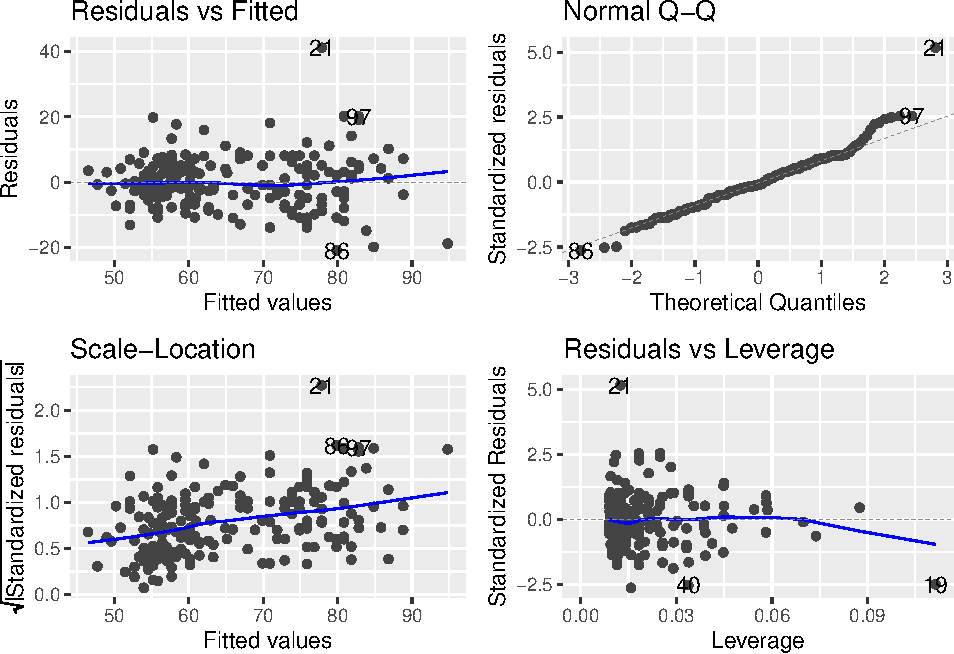
\includegraphics{Experimental-Design,-ANOVA-and-ANCOVA_files/figure-latex/unnamed-chunk-40-1.pdf}

OK. Let's walk through the three core diagnostics.

In the upper left, we are evaluating the systematic part of the model - are there any systematic departures from the linear model we've speficied? Are there interactions missing or specific non-linearities? Nope.

In the upper right, we are evaluating the normality of the residuals. These too look pretty good. If you notice, event though there are some deviations, but the pattern is that the deviations move away from the line but `come back' at the very ends. This is typical of normally distributed residuals.

In the lower left, we are evaluating the assumption of a constant mean-variance relationship. Oops. Remember, we are expecting something that does not show a trend at all. Even without the panic lines, this looks like the variance (y-axis) is increasing with the mean (x-axis).

\hypertarget{dealing-with-the-mean-variance-breakdown.}{%
\subsection{Dealing with the mean-variance breakdown.}\label{dealing-with-the-mean-variance-breakdown.}}

The above issue is one we can deal with via a \emph{transformation}.

Let's start with the facts\ldots. When the \emph{variance increases with the mean}, a transformation that can work is the \emph{logarithm of the continuous variables}.

There is a short section in the (APS 240 reading){[}\url{https://dzchilds.github.io/stats-for-bio/data-transformations.html\#trans-types}{]} to explore. Please do read this summary about transformations, and bookmark it for the future. It is very handy.

A question that routinely comes up is whether transformations are `changing the data'. Rather than focusing on this, we offer the following interpretation. Linear models fit by \texttt{lm()} carry a set of assumptions (our focus on the three panels using autoplot). If these are not met, we can not trust our inference (F-testing).

\begin{quote}
Most biological data are unlikely to conform perfectly to all the assumptions, but experience has shown (fortunately) that t-tests, ANOVAs and regressions are generally quite robust---they perform reasonably well with data that deviate to some extent from the assumptions of the tests. However, in some cases residuals are clearly very far from normal, or variances change a lot across groups - from (APS 240){[}\url{https://dzchilds.github.io/stats-for-bio/data-transformations.html\#transforms-introduction}{]}.
\end{quote}

But if there are real problems, we can use transformations. They do not `change the data' instead, they retain the relationships between the data points, but put everything on a difference scale so that we can use the power of the linear model to answer the question. The tricky thing is how do we report our insights to the reader back on the original `response' scale. We'll get to that. But rest assured, transformations don't change the data.

So, here are the data where we transform both continuous variables - the continuous response variable and the continuous explanatory variable.

\begin{Shaded}
\begin{Highlighting}[]
\CommentTok{\# re{-}plot with log{-}log}
\FunctionTok{ggplot}\NormalTok{(}\AttributeTok{data =}\NormalTok{ Davis, }\FunctionTok{aes}\NormalTok{(}\AttributeTok{x =} \FunctionTok{log}\NormalTok{(height), }\AttributeTok{y =} \FunctionTok{log}\NormalTok{(weight), }\AttributeTok{col =}\NormalTok{ sex))}\SpecialCharTok{+}
  \FunctionTok{geom\_point}\NormalTok{()}\SpecialCharTok{+}
  \FunctionTok{geom\_smooth}\NormalTok{(}\AttributeTok{method =}\NormalTok{ lm, }\AttributeTok{se =} \ConstantTok{FALSE}\NormalTok{)}
\end{Highlighting}
\end{Shaded}

\begin{verbatim}
## `geom_smooth()` using formula 'y ~ x'
\end{verbatim}

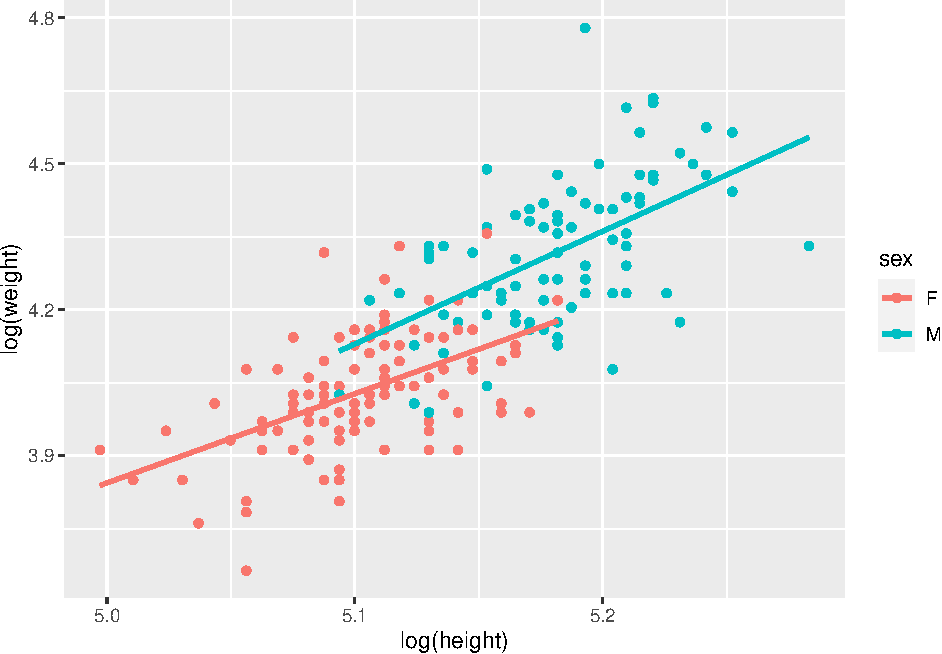
\includegraphics{Experimental-Design,-ANOVA-and-ANCOVA_files/figure-latex/unnamed-chunk-41-1.pdf}

OK. The patterns are still there. And let's see what happens with the model and assumptions now!

\begin{Shaded}
\begin{Highlighting}[]
\CommentTok{\# fit the model {-} note we can specify the transformation RIGHT IN THE MODEL}
\NormalTok{mod\_Davis\_log }\OtherTok{\textless{}{-}} \FunctionTok{lm}\NormalTok{(}\FunctionTok{log}\NormalTok{(weight) }\SpecialCharTok{\textasciitilde{}} \FunctionTok{log}\NormalTok{(height) }\SpecialCharTok{*}\NormalTok{ sex, }\AttributeTok{data =}\NormalTok{ Davis)}

\CommentTok{\# check the new residuals}
\FunctionTok{autoplot}\NormalTok{(mod\_Davis\_log)}
\end{Highlighting}
\end{Shaded}

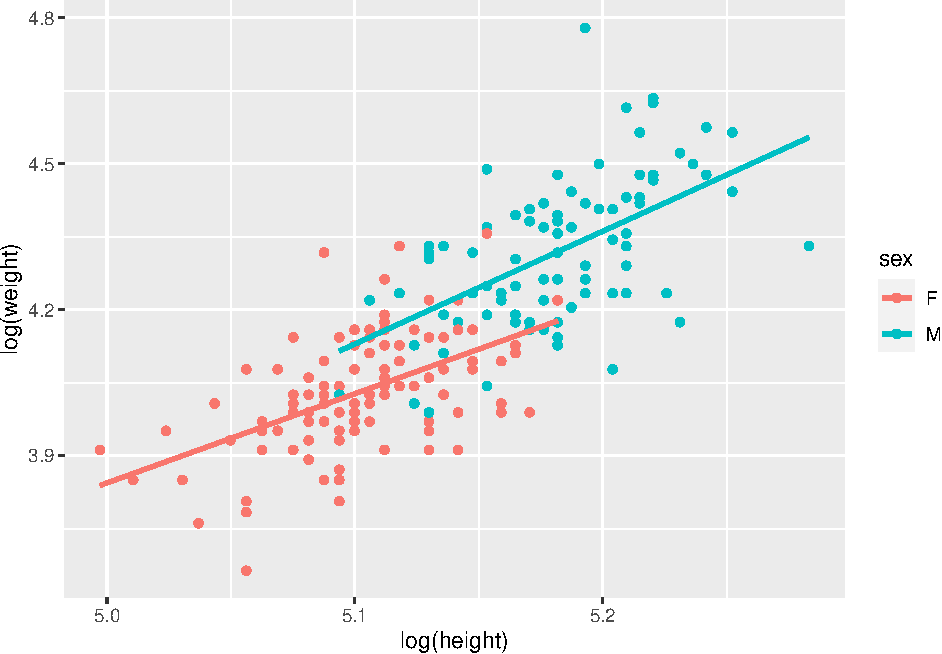
\includegraphics{Experimental-Design,-ANOVA-and-ANCOVA_files/figure-latex/unnamed-chunk-42-1.pdf}

The scale-location plot is definitely flatter - you can tell by the range on the y-axis of the scale-location plot. So, with this transformation, we can now move to evaluating the model. You are probably thinking about what it means to analyse the data on the log-log axis\ldots. we will come to that shortly.

\hypertarget{making-inference-on-the-ancova}{%
\subsection{Making inference on the ANCOVA}\label{making-inference-on-the-ancova}}

The next step is to use the detail in the ANOVA table - yes, we use the same \texttt{anova()} function to build an anova table to explore the results of an ANCOVA.

Let's revisit our initial guesses and work through what the model is telling us:

\begin{enumerate}
\def\labelenumi{\arabic{enumi}.}
\tightlist
\item
  Males are heavier than females (what is the difference in the intercepts?)
\item
  The effect of height on weight is positive (the slope(s) are positive, not negative)
\item
  There might be a difference in slopes - the Male line is steeper.
\end{enumerate}

Together, the graph and these guesses lead to a feeling that \emph{the effect of height on weight varies by sex}.

\begin{Shaded}
\begin{Highlighting}[]
\FunctionTok{anova}\NormalTok{(mod\_Davis\_log)}
\end{Highlighting}
\end{Shaded}

\begin{verbatim}
## Analysis of Variance Table
## 
## Response: log(weight)
##                  Df Sum Sq Mean Sq  F value    Pr(>F)    
## log(height)       1 4.6643  4.6643 357.4735 < 2.2e-16 ***
## sex               1 0.3446  0.3446  26.4115 6.647e-07 ***
## log(height):sex   1 0.0144  0.0144   1.1038    0.2947    
## Residuals       196 2.5574  0.0130                       
## ---
## Signif. codes:  0 '***' 0.001 '**' 0.01 '*' 0.05 '.' 0.1 ' ' 1
\end{verbatim}

Howwever\ldots. The table tells us that there is \emph{no evidence for an interaction}. The last line of this table contains the p-value for the interaction. It is testing the null hypothesis that the slopes are the same. We can not reject this null hypothesis. There is no evidence that allowing the slopes for Males and Females be different is supported. That's the answer to guess 3 above. It is also the answer to our question: does the effect of Height on Weight vary by Sex. \emph{Nope.}

However, we do detect \emph{main effects} of height and sex. This means that each of these DOES have an effect - but we say the effects are additive.

Great. What this means is that the data, despite the pattern our eye sees, can not be distinguished from the pattern in the picture in the lower left.

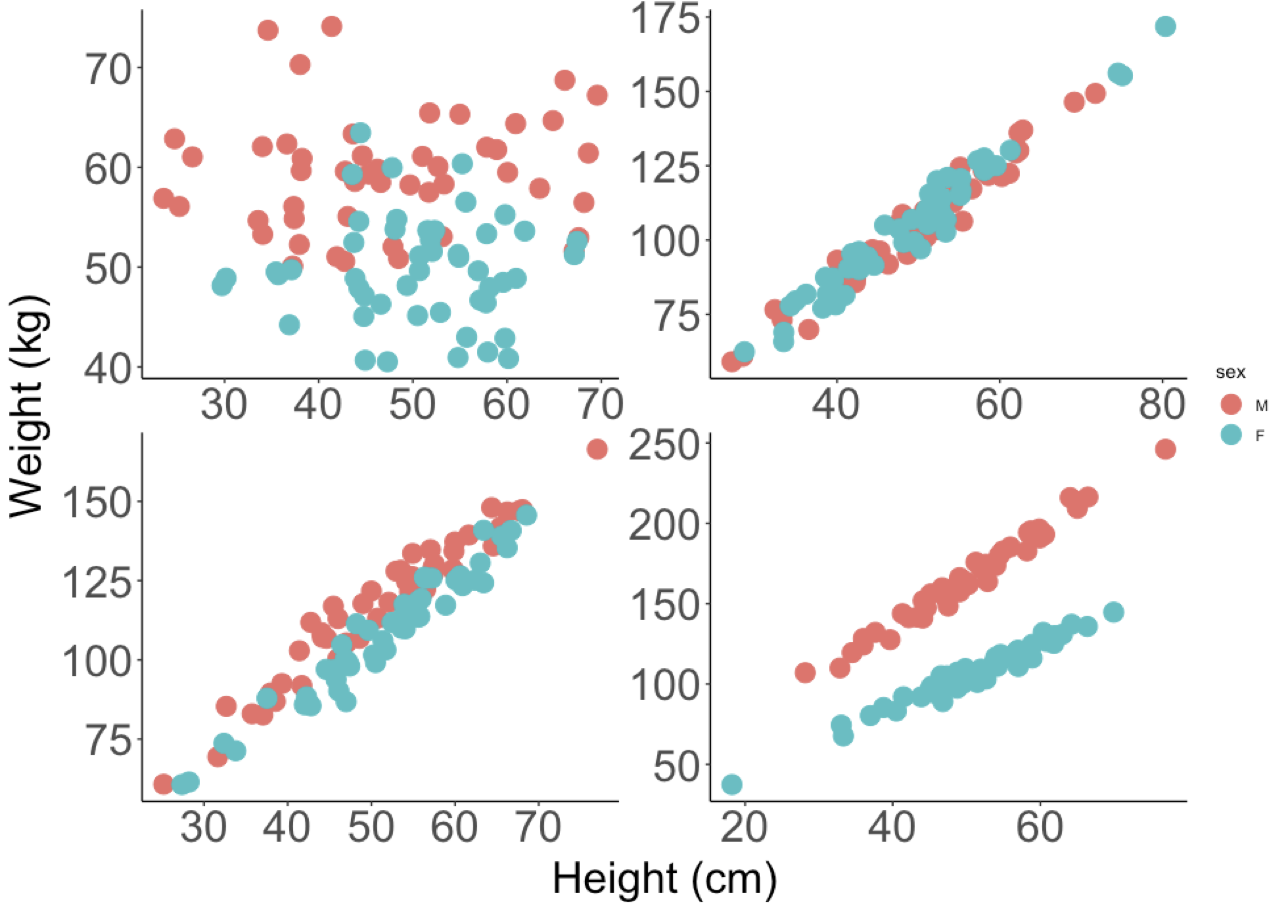
\includegraphics[width=17.89in]{images/ANCOVA_1}

There is a slope associated with Height (we don't know whether it's positive or not, but we think it is), and there is an effect of sex (we don't know whether Males are heavier yet). What we can say, with confidence, is this.

\begin{quote}
The effect of height on weight did not vary by sex (F = 1.01, df = 1,196, p = 0.29). The effect of sex (F, df, p) and height (F, df, p) are thus additive on Weight.
\end{quote}

Let's work sequentially to read the table now:

When we allow for a common slope associated with \texttt{log(Height)}, we capture \(4.66\) units of variation in \texttt{log(weight)}, which when compared to the \(0.013\) units of variation left over (residual MSE), is a lot. The F-value is thus BIG and the p-value small. When we allow for an effect of Sex to define different average \texttt{log(weight)}, this too is important as it captures \(0.344\) units of variation, which comparied to the \(0.013\) units in the residual, is also big (Big F, small P).

However, when we allow for the slopes caused by \texttt{log(height)} to vary with \texttt{sex}, this captures very little additional variation with respect to the residual variation (\(0.014\) comprared to \(0.013\)) hence a small F and a large P for this term.

\hypertarget{the-summary-table-the-actual-slopes-and-making-sense-of-the-log-stuff.}{%
\subsection{The summary table, the actual slopes and making sense of the log stuff.}\label{the-summary-table-the-actual-slopes-and-making-sense-of-the-log-stuff.}}

Let's start investigating the details via the \texttt{summary} table:

\begin{Shaded}
\begin{Highlighting}[]
\FunctionTok{summary}\NormalTok{(mod\_Davis\_log)}
\end{Highlighting}
\end{Shaded}

\begin{verbatim}
## 
## Call:
## lm(formula = log(weight) ~ log(height) * sex, data = Davis)
## 
## Residuals:
##      Min       1Q   Median       3Q      Max 
## -0.29310 -0.06543 -0.00592  0.07420  0.43410 
## 
## Coefficients:
##                  Estimate Std. Error t value Pr(>|t|)    
## (Intercept)       -5.3202     1.6016  -3.322  0.00107 ** 
## log(height)        1.8329     0.3138   5.841 2.13e-08 ***
## sexM              -2.3724     2.3765  -0.998  0.31936    
## log(height):sexM   0.4852     0.4618   1.051  0.29473    
## ---
## Signif. codes:  0 '***' 0.001 '**' 0.01 '*' 0.05 '.' 0.1 ' ' 1
## 
## Residual standard error: 0.1142 on 196 degrees of freedom
## Multiple R-squared:  0.6626, Adjusted R-squared:  0.6575 
## F-statistic: 128.3 on 3 and 196 DF,  p-value: < 2.2e-16
\end{verbatim}

This table reports on the \emph{treatment contrasts} we introduced earlier this semester. Let's walk through the details.

The first two rows correspond to one of the sexes. Can you identify which one? The hint is looking at the other rows. They have an M after them. M comes after F (F is first in the alphabet). So the first two rows correspond to \emph{the intercept and slope of the Females}.

You may be asking why the intercept is a negative number. A simple look back at the range of the x-axis should answer this\ldots{} the y intercept occurs at x = 0, right?

You should understand, from the principles of an equation for a line, the following:

\begin{quote}
the effect of height on weight for females is \texttt{log(weightF)\ =\ -5.32\ +\ 1.82*log(heightF)}.
\end{quote}

OK\ldots{} let's interpret what the next two lines mean. The third line is labelled \texttt{SexM.} The fourth is labelled \texttt{logHeight:SexM}. Any guesses as to which is associated with the slope and which the intercept?

One trick, again, is to recognise the syntax -\textgreater{} the presence of the \texttt{:} is indicative of the interaction which is the thing that lets slopes vary. So, \texttt{SexM} is about intercepts and \texttt{logHeight:SexM} is about slopes. But what are they?

Recall from previous work that \emph{treatment contrasts are about DIFFERENCES}. Thus, the \texttt{sexM} term is a difference between the female and male intercept! The \texttt{logHeight:SexM} is about the difference between the female and male slopes!

This allows the following maths to be worked out \ldots.

\texttt{log(weightF)\ =\ -5.32\ +\ 1.82*log(heightF)}

\texttt{log(weightM)\ =\ (-5.32-2.37)\ +\ (1.82+0.48)*(log(heightF))}

However, we know that the \(0.48\) increase in the slope is not signficant, and as a result, the -2.37 increase in the intercept moving from Female to Male is also not a significant change

\hypertarget{specifying-the-equations-supported-by-the-model.}{%
\subsection{Specifying the equations supported by the model.}\label{specifying-the-equations-supported-by-the-model.}}

In order to identify the equations supported by the model - e.g.~the equations associated with the estimation of teo lines with different intercepts and the same slope, we can refit the model to reflect the ADDITIVE effects only, replacing the \texttt{*} with the \texttt{+}.

\begin{Shaded}
\begin{Highlighting}[]
\NormalTok{mod\_Davis\_log2 }\OtherTok{\textless{}{-}} \FunctionTok{lm}\NormalTok{(}\FunctionTok{log}\NormalTok{(weight) }\SpecialCharTok{\textasciitilde{}} \FunctionTok{log}\NormalTok{(height) }\SpecialCharTok{+}\NormalTok{ sex, }\AttributeTok{data =}\NormalTok{ Davis)}
\FunctionTok{summary}\NormalTok{(mod\_Davis\_log2)}
\end{Highlighting}
\end{Shaded}

\begin{verbatim}
## 
## Call:
## lm(formula = log(weight) ~ log(height) + sex, data = Davis)
## 
## Residuals:
##      Min       1Q   Median       3Q      Max 
## -0.28714 -0.06906 -0.00978  0.07615  0.43717 
## 
## Coefficients:
##             Estimate Std. Error t value Pr(>|t|)    
## (Intercept) -6.46349    1.17541  -5.499 1.18e-07 ***
## log(height)  2.05688    0.23030   8.931 2.99e-16 ***
## sexM         0.12417    0.02417   5.138 6.66e-07 ***
## ---
## Signif. codes:  0 '***' 0.001 '**' 0.01 '*' 0.05 '.' 0.1 ' ' 1
## 
## Residual standard error: 0.1143 on 197 degrees of freedom
## Multiple R-squared:  0.6607, Adjusted R-squared:  0.6573 
## F-statistic: 191.8 on 2 and 197 DF,  p-value: < 2.2e-16
\end{verbatim}

Right, now we get our expected pattern where the intercepts are different but the slope is the same:

\texttt{log(weightF)\ =\ -6.46\ +\ 2.05*log(heightF)}

\texttt{log(weightM)\ =\ (-6.46\ +\ 0.12)\ +\ 2.05*log(heightF)}

We can see the common slope and the slightly higher average weight (\(0.12\) units!) of males.

\hypertarget{making-even-more-inference-and-drawing-the-picture}{%
\subsection{Making even more inference and drawing the picture}\label{making-even-more-inference-and-drawing-the-picture}}

OK, lets use a variation on our plotting tricks from the regression module (week 6) to get a nice picture.

\begin{Shaded}
\begin{Highlighting}[]
\CommentTok{\# first create a data frame to use that combines the raw data}
\CommentTok{\# with the predictions from the model.}

\CommentTok{\# note that the model is the ADDITIVE model, for plotting}
\CommentTok{\# step 1: make a copy of the raw data}
\CommentTok{\# step 2: use mutate to add the fitted values (at each value of height (x{-}axis) where we have measured data)}
\NormalTok{plotThis }\OtherTok{\textless{}{-}}\NormalTok{ Davis }\SpecialCharTok{\%\textgreater{}\%}
  \CommentTok{\# ... a column of numbers of predicted weight using the model}
  \FunctionTok{mutate}\NormalTok{(}\AttributeTok{predWeight =} \FunctionTok{predict}\NormalTok{(mod\_Davis\_log2))}

\CommentTok{\# check it out.}
\FunctionTok{head}\NormalTok{(plotThis)}
\end{Highlighting}
\end{Shaded}

\begin{verbatim}
##   sex weight height repwt repht predWeight
## 1   M     77    182    77   180   4.364677
## 2   F     58    161    51   159   3.988326
## 3   F     53    161    54   158   3.988326
## 4   M     68    177    70   175   4.307379
## 5   F     59    157    59   155   3.936578
## 6   M     76    170    76   165   4.224381
\end{verbatim}

You can see we have a fourth column now\ldots. these are predictions (also known as fitted values) of \texttt{log(weight)} as a function of \texttt{log(height)} using the additive model, \emph{at each of the originally measured height values in the data frame}.

We can actually use this data frame to generate the picture that represents the output of the statistical model.

\begin{Shaded}
\begin{Highlighting}[]
\CommentTok{\# Step 3: make a figure with lines from the model predictions}
\CommentTok{\# Step 4: add the raw data points from the original dataset}
\CommentTok{\# }\AlertTok{NOTE}\CommentTok{! pay attention to where we are using log()!}
\FunctionTok{ggplot}\NormalTok{(plotThis, }\FunctionTok{aes}\NormalTok{(}\AttributeTok{x =} \FunctionTok{log}\NormalTok{(height), }\AttributeTok{y =}\NormalTok{ predWeight, }\AttributeTok{col =}\NormalTok{ sex))}\SpecialCharTok{+}
  \FunctionTok{geom\_line}\NormalTok{()}\SpecialCharTok{+}
  \CommentTok{\# now add the raw data note}
  \FunctionTok{geom\_point}\NormalTok{(}\FunctionTok{aes}\NormalTok{(}\AttributeTok{x =} \FunctionTok{log}\NormalTok{(height), }\AttributeTok{y =} \FunctionTok{log}\NormalTok{(weight)))}
\end{Highlighting}
\end{Shaded}

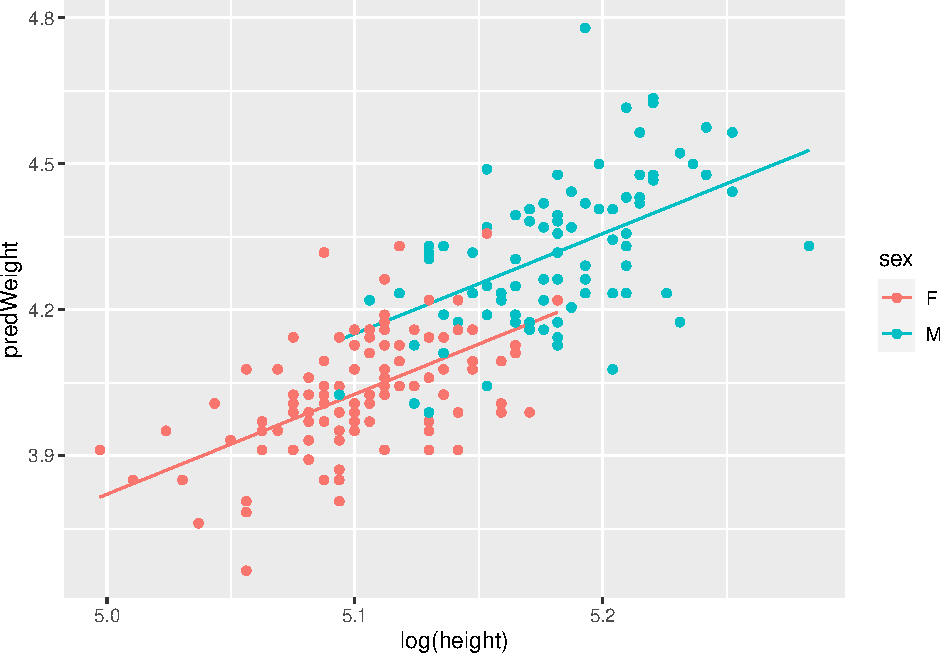
\includegraphics{Experimental-Design,-ANOVA-and-ANCOVA_files/figure-latex/unnamed-chunk-48-1.pdf}

Great. Now we can see that the full model (mod\_Davis\_log) told us. The lines are parallel. There is no interaction. In fact, we can do a bit more here. Remember that the model says

For women \(log(weight)= -6.46 + 2.05 * log(height)\)
For men \(log(weight)= (-6.46 + 0.12) + 2.05 * log(height)\)

Because we are in log land, we can do some clever maths: We know that

\(log(weight Female) - log(weight Male) = - 0.12\)

(this is the treatment contrast for the intercept). We also know (please memorise) that the \emph{difference between logs is equal to the log of the ratio}:

\(log(weightF/weightM) = -0.12\)

Finally, we can convert both sides to non-log by exponentiating:

\(exp(log(weightF/weightM)) = exp(-0.12) = 0.88\)

What does this mean? At any given height, female weight is 88\% of a males (e.g.~12\% lower). Cool! That's one of the benefits of log-log linear relationships. \emph{The ratio of the categories in log-log land directly translates to a percent difference between the groups}. It's also worth noting that the height slope is \textasciitilde2, which suggests\ldots{} yes\ldots{} because we are in log-land, that weight scales with \(height^2\).

\hypertarget{some-general-principles-for-anova-and-ancova-modelling.}{%
\section{Some General Principles for ANOVA and ANCOVA modelling.}\label{some-general-principles-for-anova-and-ancova-modelling.}}

\hypertarget{ancova-and-2-way-anova-is-always-comparing-the-interaction-model-against-the-additive-model}{%
\subsection{ANCOVA (and 2-way ANOVA) is always comparing the interaction model against the additive model!}\label{ancova-and-2-way-anova-is-always-comparing-the-interaction-model-against-the-additive-model}}

This figure highlights the various \texttt{lm()} models and their interpretations/assumptions associated with the pieces of an ANCOVA dataset. This is a way to envision all of the potential linear relationships among the variables that might arise in an experiment with a continuous and categorical explanatory variable.

\begin{quote}
Note that just because your data looks like a particular pattern doesn't mean you should use that model. Your statistical model should be driven by your question and original design.
\end{quote}

\begin{figure}
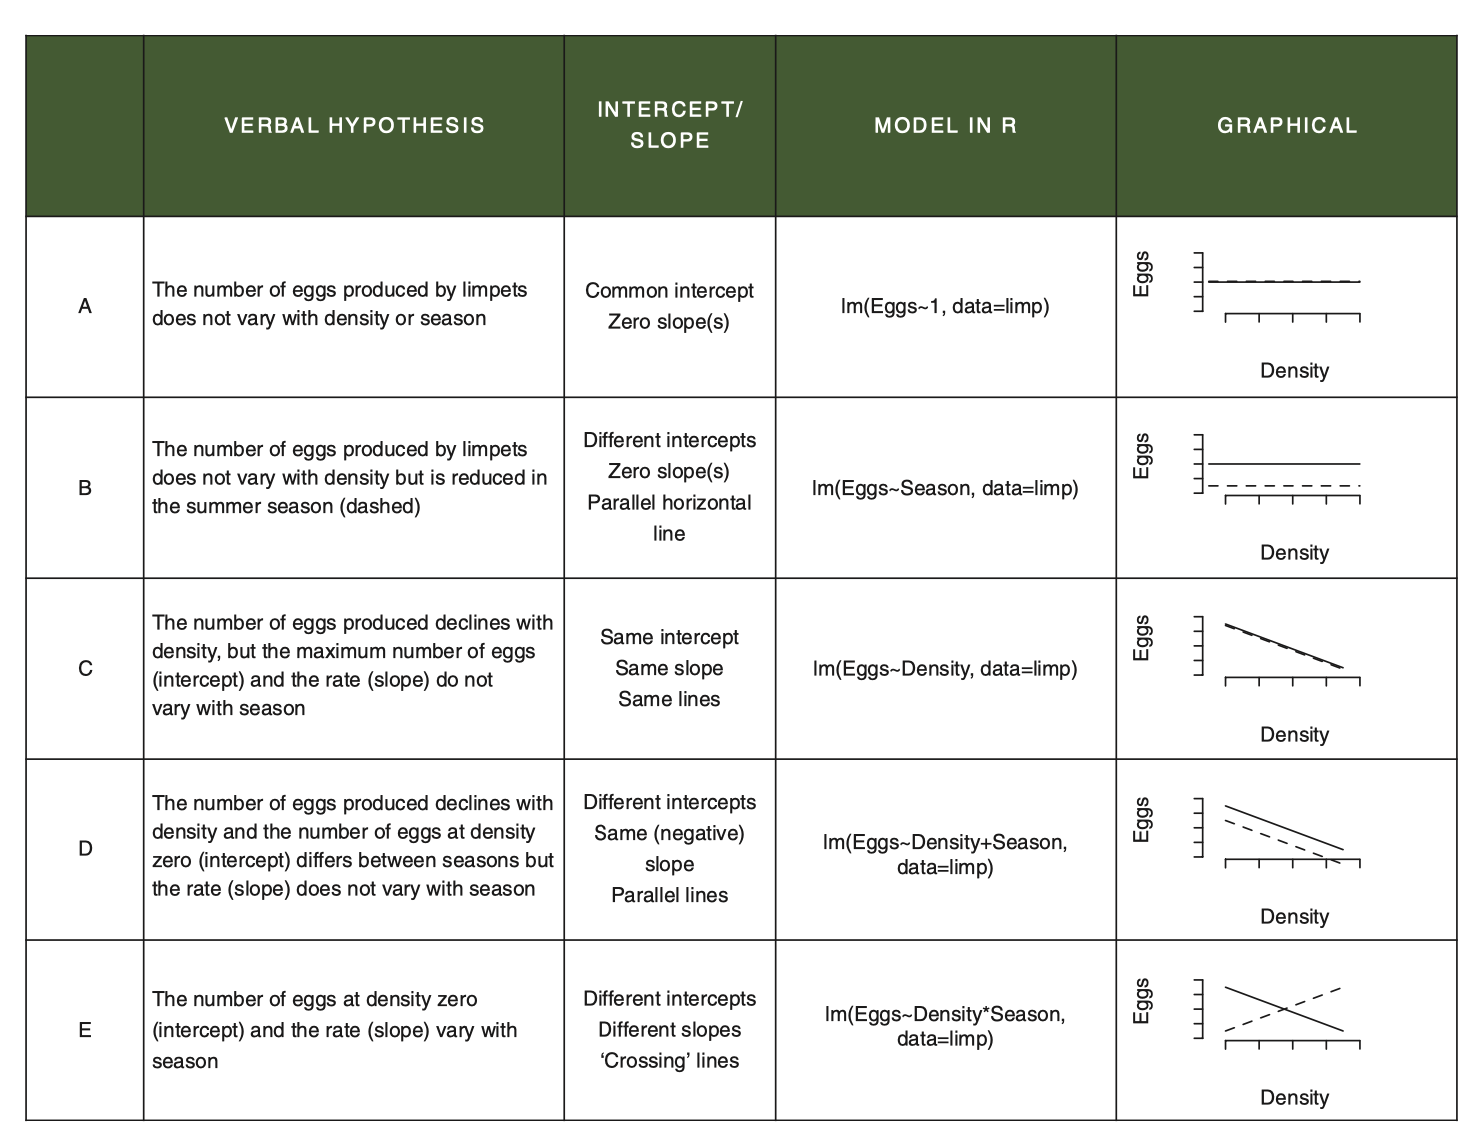
\includegraphics[width=20.56in]{images/GSwithR_Grid} \caption{From Getting Started with R, 2nd Edition, OUP}\label{fig:unnamed-chunk-49}
\end{figure}

For example, if you design a study with an ANCOVA question in mind, you are always starting your analysis with the question of whether the effect of X on Y varies by Z. Thus, ANCOVA always starts with comparing the interaction (model E) against the additive model (model D).

\begin{quote}
Proof: If we compare the additive model and the model with the interaction, we are \emph{specifically} testing for whether allowing the slopes to vary by sex \emph{explains additional variation} above and beyond the main, additive effects of height and sex. To do this, we use the \texttt{anova()} function, but pass it two models instead of one! This does what is called a \emph{Liklihood Ratio Test} comparing the two models. Remembering that the difference between the \texttt{*} model and the \texttt{+} model is just the presence/absence of the interaction term, this \texttt{anova()} comparison evaluates how much more variation is explained by the interaction, after the additive effects have been modelled. In the follow code, compare the result of the first test to the \emph{last line} of the second. This proves that when we fit model E, the test for the interaction is actually a comparison of model E with model D!
\end{quote}

\begin{Shaded}
\begin{Highlighting}[]
\FunctionTok{anova}\NormalTok{(mod\_Davis\_log, mod\_Davis\_log2)}
\end{Highlighting}
\end{Shaded}

\begin{verbatim}
## Analysis of Variance Table
## 
## Model 1: log(weight) ~ log(height) * sex
## Model 2: log(weight) ~ log(height) + sex
##   Res.Df    RSS Df Sum of Sq      F Pr(>F)
## 1    196 2.5574                           
## 2    197 2.5718 -1 -0.014402 1.1038 0.2947
\end{verbatim}

\begin{Shaded}
\begin{Highlighting}[]
\FunctionTok{anova}\NormalTok{(mod\_Davis\_log)}
\end{Highlighting}
\end{Shaded}

\begin{verbatim}
## Analysis of Variance Table
## 
## Response: log(weight)
##                  Df Sum Sq Mean Sq  F value    Pr(>F)    
## log(height)       1 4.6643  4.6643 357.4735 < 2.2e-16 ***
## sex               1 0.3446  0.3446  26.4115 6.647e-07 ***
## log(height):sex   1 0.0144  0.0144   1.1038    0.2947    
## Residuals       196 2.5574  0.0130                       
## ---
## Signif. codes:  0 '***' 0.001 '**' 0.01 '*' 0.05 '.' 0.1 ' ' 1
\end{verbatim}

\hypertarget{a-few-parting-tricks-about-specifying-models-in-r}{%
\section{A few parting tricks about specifying models in R}\label{a-few-parting-tricks-about-specifying-models-in-r}}

We can add terms
\texttt{weight\ \textasciitilde{}\ sex\ +\ height}

Have can crossed terms (interactions)
\texttt{weight\ \textasciitilde{}\ sex\ *\ height} which is \texttt{weight\ \textasciitilde{}\ sex\ +\ \ height\ +\ sex\ :\ height}

We can remove terms
\texttt{weight\ \textasciitilde{}\ sex\ *\ height\ –\ sex\ :\ height} which is \texttt{weight\textasciitilde{}\ sex\ +\ \ height}

We can specify interations of order k among 2 or more terms:
\texttt{weight\textasciitilde{}\ (sex\ +\ height\ +\ age)\^{}2} which expands to \texttt{sex\ +\ height\ +\ age\ +\ sex\ :\ height\ +\ sex\ :\ age\ +\ age\ :\ height} (e.g.~all two way interactions among the three variables)

\end{document}
